\documentclass{jvfscript-de}
%=======================================================================================================%
%                                                                                                       %
% Dieses Skript benötigt mein Package jvftex, erhältlich unter https://github.com/vonfalkenstein/jvftex %
%                                                                                                       %
%=======================================================================================================%
\usepackage{ztstyle}
\usepackage{graphicx}
\graphicspath{ {./images/} }

%\usepackage{showframe}

\makeindex[title=Definitionen,intoc]
\DeclareNewTOC[owner=jvfscript-de,listname=Dateiverzeichnis,type=files,types=files, name=Datei]{listoffiles}
\newcounter{file}
\newcounter{video}
\renewcommand{\lecture}[1]{%
	\setcounter{video}{0}
	\stepcounter{lecture}
	\marginnote{\normalfont Vorlesung \thelecture, #1}
	\addxcontentsline{listoflectures}{section}[]{Vorlesung \thelecture{} vom #1}
}
\newcommand{\file}[1]{%
	\stepcounter{file}
	\marginnote{\normalfont Datei \thefile: #1}
	\addxcontentsline{listoffiles}{section}[]{Datei \thefile{} - {#1}}
}
\newcommand{\video}{%
	\stepcounter{video}
	\marginnote{\normalfont Video \thelecture\_\thevideo}
}
\newcommand{\filevideo}[1]{%
	\stepcounter{file}
	\stepcounter{video}
	\marginnote{\normalfont Datei \thefile: #1,\\Video \thelecture\_\thevideo}
	\addxcontentsline{listoffiles}{section}[]{Datei \thefile{} - {#1}}
}
\newcommand{\lecturefile}[2]{%
	\stepcounter{file}
	\stepcounter{lecture}
	\marginnote{\normalfont Vorlesung \thelecture, #1, Datei \thefile: #2}
	\addxcontentsline{listoflectures}{section}[]{Vorlesung \thelecture{} vom #1}
	\addxcontentsline{listoffiles}{section}[]{Datei \thefile{} - {#2}}
}
\newcommand{\lecturevideo}[1]{%
	\setcounter{video}{0}
	\stepcounter{lecture}
	\stepcounter{video}
	\marginnote{\normalfont Vorlesung \thelecture, #1, Video \thelecture\_\thevideo}
	\addxcontentsline{listoflectures}{section}[]{Vorlesung \thelecture{} vom #1}
}
\newcommand{\lecturefilevideo}[2]{%
\setcounter{video}{0}
\stepcounter{file}
\stepcounter{lecture}
\stepcounter{video}
\marginnote{\normalfont Vorlesung \thelecture, #1, Datei \thefile: #2, Video \thelecture\_\thevideo}
\addxcontentsline{listoflectures}{section}[]{Vorlesung \thelecture{} vom #1}
\addxcontentsline{listoffiles}{section}[]{Datei \thefile{} - {#2}}
}

%\renewcommand{\thechapter}{\S \arabic{chapter}}
%\renewcommand{\thesection}{\arabic{chapter}.\arabic{section}}
\renewcommand{\thethm}{\arabic{chapter}.\arabic{thm}}

\hypersetup{
	pdftitle={Vorlesungsskript Zahlentheorie}
}



%\includeonly{./lectures/cpt10}

\usetikzlibrary{patterns}
%\usepackage[dvipsnames]{xcolor}
\usepackage{pgfplots}

\begin{document}
\frontmatter
	\maketitle
	\pagestyle{plain}
	\begingroup
	\let\clearpage\relax
	\tableofcontents
	\listoflectures
	\listoffiles
	\endgroup
\newpage

Dieses Skript stellt keinen Ersatz für die Vorlesungsnotizen von Prof. Schindler dar und wird nicht nochmals von ihr durchgesehen. Im Grunde sind das hier nur meine persönlichen Mitschriften, ich garantiere also weder für Korrektheit noch Vollständigkeit und werde ggf. noch weitere Beispiele und Anmerkungen einfügen. Beweise werde ich in der Regel nicht übernehmen (weil das in \LaTeX{} einfach keinen Spaß macht).

Falls Ihr Korrekturanmerkungen habt könnt Ihr mir gern bei \href{https://studip-ecampus.uni-goettingen.de/dispatch.php/profile?username=n.sennewald}{Stud.IP} schreiben oder direkt im \href{https://github.com/vonfalkenstein/Vorlesungsmitschrift-Zahlentheorie}{GitHub Repository} einen pull request machen (was für mich deutlich weniger umständlich ist als der Weg über Stud.IP).\\\\
glhf,\\
Alex

\vspace{\fill}
\begin{quote}
	"Die Zahlentheorie ist nützlich, weil man mit ihr promovieren kann."
\end{quote}\hspace{\fill} --Edmund Landau
\vspace{\fill}


\mainmatter
\pagestyle{scrheadings}
	
	\chapter{Primzahlen - Bausteine der ganzen Zahlen}\lecturefilevideo{13.04.2021}{Primzahlen \& Teilbarkeit}

%\[ \begin{tikzcd}
%	&&&G/\ker f \arrow{ddr}{\iota}&\\
%	\\
%	\ker f \arrow{rr}{\kappa}&& G \arrow{rr}{f} \arrow{uur}{\pi}& & H
%\end{tikzcd} \]

Wo ergeben sich für uns in der Zahlentheorie Unterschiede, wenn wir über $\Z$ anstatt über $\Q$ arbeiten?

\begin{exmp*}
	Seien $a,b \in \Z$, $a\neq 0$. Dann hat die Gleichung
	\[ ax = b \]
	nicht immer eine Lösung $x \in \Z$.
\end{exmp*}

\begin{defn*}[Teiler]\index{Teiler}
	Seien $a,b \in \Z$. Wir sagen, dass \emph{$\emph{a}$ ein Teiler von $\emph{b}$ ist} ($a \mid b$), falls es eine ganze Zahl $x \in \Z$ gibt mit $ax = b$.
\end{defn*}

\begin{lem}\autolabel
	Seien $a,b,c,d \in \Z$.
	\begin{enumerate}[label={\roman*})]
		\item Falls $d \mid a$ und $d \mid b$, dann $d \mid a+b$.
		\item Ist $d \mid a$, dann auch $d \mid ab$.
		\item Ist $d \mid a$, dann gilt $db \mid ab$.
		\item Gilt $d \mid a$ und $a \mid b$, dann $d \mid b$.
		\item Ist $a \neq 0$ und $d \mid a$, dann gilt $|d| \leq |a|$.
	\end{enumerate}
\end{lem}

\begin{rem*}
	Eine ganze Zahl $a \neq 0$ hat höchstens endlich viele Teiler.
\end{rem*}

\begin{thm}[Teilen mit Rest]\autolabel
	Seien $a,b \in \Z, b > 0$. Dann gibt es $q,r \in \Z$ mit
	\[ a = bq + r, \ 0 \leq r < b. \]
\end{thm}

\begin{defn*}[Primzahl]\index{Primzahl}\video
	Eine ganze Zahl $p > 1$, die genau zwei positive Teiler hat (1 und sich selbst), nenn wir \emph{Primzahl}.
\end{defn*}

\begin{exmp*}
	\( 2,3,5,7,11,13,17,19,23,29,31,\dotsc \)
\end{exmp*}

\begin{lem}\autolabel
	Sei $n \in \N, n > 1$ und sei $p>1$ der kleinste positive Teiler von $n$. Dann ist $p$ eine Primzahl. Ist außerdem $n$ nicht prim, dann gilt $p \leq \sqrt{n}$.
\end{lem}

\begin{rem*}
	Diese Eigenschaft findet Anwendung im \emph{Sieb von Eratosthenes}. Dies ist ein einfacher Algorithmus, um schnell alle Primzahlen bis $n$ zu finden. Hierfür definieren wir zunächst die Menge \( A = \{z \in \Z \mid 2 \leq z \leq n\} \). Durch Lemma \ref{1.3} genügt es, zusätzlich lediglich die Menge $B = \{k \cdot p \mid k \in \Z, p \leq \sqrt{n} \ \text{prim}\}$, also alle Primzahlen $p \leq \sqrt{n}$ und deren Vielfache zu betrachten. Die Differenz $A \setminus B$ beinhaltet dann nur noch alle Primzahlen $\sqrt{n} \leq p \leq n$.
\end{rem*}

\begin{thm}[Euklid]\autolabel
	Es gibt unendlich viele Primzahlen.
\end{thm}

\begin{thm}[Hauptsatz der Arithmetik, Primfaktorzerlegung]\autolabel
	Jede natürliche Zahl $n > 1$ kann auf eindeutige Weise als Produkt
	\[ n = p_1^{k_1} \cdot p_2^{k_2} \dotsm p_r^{k_r} \]
	mit $k_1, \dotsc, k_r \in \N$ und $p_1 < p_2 < \dots < p_r$ Primzahlen geschrieben werden.
\end{thm}

\begin{lem}\video\autolabel
	Seien \( a,b, p \in \N \) und $p$ eine Primzahl. Angenommen $p \mid ab$, dann gilt $p \mid a$ oder $p \mid b$.
\end{lem}

\begin{cor}\autolabel
	Seien $a_1,\dotsc,a_n \in \N$ und $p$ eine Primzahl mit $p \mid a_1 \dotsm a_n$. Dann $\existss 1 \leq i \leq n$ mit $p \mid a_i$.
\end{cor}

\begin{thm}\autolabel
	Seien $a, b \in \N$ mit Primfaktorzerlegungen
	\[ a = p_1^{a_1} \cdot p_2^{a_2} \dotsm p_r^{a_r},\quad b = p_1^{b_1} \cdot p_2^{b_2} \dotsm p_r^{b_r} \]
	mit $p_1, \dotsc,r_p$ Primzahlen, $p_i \neq p_j$ für $i \neq j$ und $a_i,b_i \geq 0\ \foralll i$. Dann gilt genau dann \( b \mid a \), wenn \( b_i \leq a_i \ \foralll i \).
\end{thm}

\subsection*{Der größte gemeinsame Teiler}\video

\begin{defn*}[größter gemeinsamer Teiler]\index{größter gemeinsamer Teiler}
	Seien $a,b \in \N$. Der \emph{größte gemeinsame Teiler von $\emph{a}$ und $\emph{b}$} ist der größte Teiler $d$ mit $d \mid a$ und $d \mid b$. Wir schreiben $\ggt(a,b) = d$ (im englischen $\gcd(a,b)$).
\end{defn*}

\begin{rem*}
Seien $a = p_1^{a_1} \cdot p_2^{a_2} \dotsm p_r^{a_r},\quad b = p_1^{b_1} \cdot p_2^{b_2} \dotsm p_r^{b_r}$ mit $p_1, \dotsc,r_p$ Primzahlen, $p_i \neq p_j$ für $i \neq j$ und $a_i,b_i \geq 0\ \foralll 1 \leq i \leq r$, und $d \in \N$ mit $ d = p_1^{d_1} \cdot p_2^{d_2} \dotsm p_r^{d_r}$, wobei $d_i \geq 0 \ \foralll 1 \leq i \leq r$. Angenommen $d \mid a$ und $d \mid b$, dann $d_i \leq a_i,b_i \ \foralll 1 \leq i \leq r$. Ist $d = \ggt(a,b)$, dann gilt $d_i = \min(a_i,b_i) \ \foralll 1 \leq i \leq r$ und 
$$\ggt(a,b) = p_1^{\min(a_1,b_1)} \cdot p_2^{\mid(a_2,b_2)} \dotsm p_r^{\min(a_r,b_r)}.$$
\end{rem*}

\begin{lem}\autolabel
	Seien $a,b,c,d \in \N$.
	\begin{enumerate}[label={\roman*})]
		\item Ist $d \mid a$ und $d \mid b$, dann $d \mid \ggt(a,b)$.
		\item Angenommen $b \mid ac$ und $\ggt(a,b) = 1$. Dann gilt $b \mid c$.
		\item Sei $a \mid c,\ b \mid c$ und $\ggt(a,b) = 1$. Dann $ab \mid c$.
		\item Sei $d = \ggt(a,b)$. Dann gilt \( \ggt \left( \frac{a}{d},\frac{b}{d} \right) = 1. \)
	\end{enumerate}
\end{lem}

\subsection*{Das kleinste gemeinsame Vielfache}

\begin{defn*}[kleinstes gemeinsames Vielfaches]\index{kleinstes gemeinsames Vielfaches}
	Seien $a,b \in \N$. Die kleinste natürliche Zahl $m$ mit $a \mid m$ und $b \mid m$ nennen wir das \emph{kleinste gemeinsame Vielfache von $\emph{a}$ und $\emph{b}$}. Wir schreiben $\kgv(a,b) = m$ (im englischen $\lcm(a,b)$).
\end{defn*}

\begin{rem*}
	Seien $a,b$ mit den gleichen Primfaktorzerlegungen wie oben. Dann
	\[ \kgv(a,b) = p_1^{\max(a_1,b_1)} \cdot p_2^{\max(a_2,b_2)} \dotsm p_r^{\max(a_r,b_r)}. \]
	Bemerke: $\max(a_i,b_i) + \min(a_i,b_i) = a_i + b_i$. Also $ab = \ggt(a,b) \cdot \kgv(a,b)$.
\end{rem*}

\begin{defn*}
	Seien \( a_1,\dotsc,a_k \in \Z \), nicht alle gleich null. Der größte gemeinsame Teiler von \( a_1,\dotsc,a_k \) ist die größte natürliche Zahl $d$, die jedes der $a_i$ teilt. Wir schreiben \( d = \ggt(a_1,\dotsc,a_k) \). Analog dazu können wir das kleinste gemeinsame Vielfache von $a_1,\dotsc, a_k$ als die kleinste positive ganze Zahl $m$ definieren, die durch jedes der $a_i$ teilbar ist, $m = \kgv(a_1,\dotsc,a_k)$.
\end{defn*}

\section*{Der Euklidische Algorithmus}\filevideo{Der Euklidische Algorithmus}

\emph{Motivation:} Seien $a,b \in \N$. Wie können wir $\ggt(a,b)$ schnell berechnen?

\begin{rem*}
	Für $a,b \in \N$ schreibe $a = qb + r$ mit $0 \leq r < b$.
	\begin{enumerate}[label={\roman*})]
		\item Ist $d \in \N$ mit $d \mit a$ und $d \mid b$, dann gilt auch $d \mid r$.
		\item Ist $d \mid b$ und $d \mid r$, dann $d \mid a$.
	\end{enumerate}
	Es folgt: $\ggt(a,b) = \ggt(b,r)$.
\end{rem*}

\begin{exmp*}
	$a = 270,\ b = 192$
	\begin{align*}
		270 &= 1 \cdot 192 + 78\\
		192 &= 2 \cdot 78 + 36\\
		78 &= 2 \cdot 36 + 6\\
		36 &= 6 \cdot 6 + 0\\
		\noalign{\centering $\implies \ggt(270,192) = \dotsc = \ggt(6,0) = 6$}
	\end{align*}
\end{exmp*}

Im Allgemeinen sieht das wie folgt aus:
\begin{align*}
	a &= q_0 b + r_1\\
	b &= q_1 r_1 + r_2\\
	r_1 &= q_2 r_2 + r_3\\
	\noalign{\centering \dots}
	r_{k-2} &= q_{k-1} r_{k-1} + r_k\\
	r_{k-1} &= q_k r_k + 0\\
	\implies \ggt(a,b) &= r_k
\end{align*}
Warum endet der Euklidische Algorithmus nach endlich vielen Schritten? In jedem Schritt gilt $0 \leq r_{j+1} < r_j \ \foralll j$. Da wir mit einer endlichen Zahl $b$ angefangen haben ist auch unser $r_1$ endlich, und da sich der Rest in jedem Schritt um mindestens 1 verkleinert sind wir nach maximal $|b|$ Schritten fertig.

Der Euklidische Algorithmus ist schnell. Sei $a > b$, dann ist $r_1 < \frac{a}{2}$. Wenn wir dies fortsetzen erhalten wir 
\begin{align*}
	r_2 &< r_1 < \frac{a}{2}\\
	r_3 &< \frac{r_1}{2} < \frac{a}{4}\\
	r_4 &< \frac{r_2}{2} < \frac{a}{4}\\
	\dots
\end{align*}
Nach Vollständiger Induktion folgt 
\[ r_m < \frac{a}{2^{\frac{m}{2}}}\qquad \foralll m>0. \]
Daher \( 1 \leq r_k < \frac{a}{2^{\frac{k}{2}}} \), also \( 2^\frac{k}{2} < a \) und somit
\[ k < 2\frac{\log a}{\log 2} \]
	\chapter{Die Teilerfunktion} \filevideo{Teilerfunktion, Kongruenzen}

\begin{defn*}[Teilerfunktion]\index{Teilerfunktion}
	Sei $n \in \N$. Wir definieren \( d(n) \) als die Zahl der positiven Teiler von $n$, d.h.
	\[ d(n) = \sum_{\substack{d \mid n \\ d \geq 1}} 1. \]
	Weiter definieren wir
	\[ S(n) = \sum_{\substack{d \mid n \\ d \geq 1 \\ d < n}} d \]
	und 
	\[ \sigma(n) = \sum_{\substack{d \mid n \\ d \geq 1}} d \]
\end{defn*}

\begin{exmp*}
	\( d(7) = 2,\ d(6) = 4 \)\\
	Sei $p$ eine Primzahl, dann gilt $d(p) = 2$ und $d(p^k) = k+1$ für $k\geq 0$.
\end{exmp*}

\begin{rem*}
	$\sigma(n) = S(n) + n$
\end{rem*}

\begin{defn*}[perfekte Zahl] \index{perfekte Zahl}
	Wir nennen eine natürliche Zahl $n$ \emph{perfekt}, falls
	\[ S(n) = n. \]
\end{defn*}

\begin{exmp*}
	$6 = 1+2+3$ ist perfekt. 28 ist perfekt.
\end{exmp*}

\begin{lem}\autolabel
	Seien $m,n \in \N$ mit $\ggt(m,n) = 1$. Dann gilt
	\[ d(mn) = d(m)d(n) \]
	und \[ \sigma(mn) = \sigma(m) \sigma(n). \]
\end{lem}

\begin{rem*}
	$d(n)$ und $\sigma(n)$ sind sogenannte \textit{multiplikative Funktionen}.
\end{rem*}

Kennt man die Primfaktorzerlegung von $n$, so lassen sich diese Funktionen sehr einfach berechnen. Wir wollen nun eine allgemeine Formel für $d(n)$ aufstellen.

Sei $n = p_1^{k_1} \dotsm p_r^{k_r}$ mit $p_1 < \dots < p_3$ Primzahlen, $k_1, \dotsm, k_r \geq 0$. Dann gilt nach Lemma \ref{2.1}
\begin{align*}
	d(n) &= d \left( p_1^{k_1} \dotsm p_r^{k_r} \right)\\
	&= d\left(p_1^{k_1}\right) \dotsm d\left(p_r^{k_r}\right)
\end{align*}
Es gilt
\[ d(p^k) = k + 1, \]
also
\[ d(n) = (k_1+1) (k_2+1) \dotsm (k_r+1). \]
Weiterhin berechnen wir
\begin{align*}
	\sigma(n) &= \sigma\left(p_1^{k_1}\right) \dotsm \sigma\left(p_r^{k_r}\right)\\
	\sigma\left(p^k\right) &= 1 +p + p^2 + \dots + p^k\\
	&= \frac{p^{k+1} -1}{p-1}
\end{align*}
Wir erhalten
\[ \sigma(n) = \frac{p_1^{k_1+1} - 1}{p_1-1} \dotsm \frac{p_r^{k_r+1}-1}{p_r-1} \]

\begin{thm}\autolabel
	Sei $n = p_1^{k_1} \dotsm p_r^{k_r}$ mit $p_1 < \dots < p_3$ Primzahlen, $k_1, \dotsm, k_r \geq 0$. Dann gilt 
	\begin{align*}
		d(n) &= \prod_{i=1}^r (k_i+1)\\
		\sigma(n) &= \prod_{i=1}^r \frac{p_i^{k_i + 1}-1}{p_i-1}.
	\end{align*}
\end{thm}

\begin{exmp*}
	\( d(25 \cdot 3) = d(25) d(3) = d(5^2) d(3) = 3 \cdot 2 = 6 \)
\end{exmp*}

\begin{rem*}
	$S(n)$ ist keine multiplikative Funktion:\\
	\( 1 = S(2)S(3) \neq S(6) = 6 \)
\end{rem*}
	\chapter{Kongruenzen}\video

\begin{exmp*}
	Die Uhr
	\incfig{3_1}{10cm}
	Der Minutenzeiger weiß nur, wie viele Minuten es nach einer vollen Stunde ist
\end{exmp*}

\begin{defn*}[Kongruenz, Kongruenzklasse]\index{Kongruenzklasse}
	Sei $M \in \N,\ M > 1,\ a,b \in \Z$. Wir sagen, dass \emph{$\emph{a}$ kongruent zu $\emph{b}$ ist modulo $\emph{M}$}, falls \( M \mid (a-b) \), schreibe \( a \equiv b \bmod M \).\\
	Sei $r \in \Z$. Die Menge aller ganzen Zahlen $x$ mit $x \equiv r \bmod M$ nennen wir die \emph{Kongruenzklasse von $\emph{r}$ modulo $\emph{M}$}.
\end{defn*}

\begin{exmp*}
	\( 7 \equiv  27 \bmod 10,\ 4 \equiv 1 \bmod 3 \)
\end{exmp*}

\begin{lem}\autolabel
	Sei $M > 1,\ M \in \N,\ a_1,a_2,b_1,b_2 \in \Z$ mit $a_1 \equiv a_2 \bmod M$ und $b_1 \equiv b_2 \bmod M$. Dann gilt
	\begin{enumerate}[label={\roman*})]
		\item $a_1 + b_1 \equiv a_2 + b_2 \bmod M$
		\item $a_1 - b_1 \equiv a_2 - b_2 \bmod M$
		\item $a_1b_1 \equiv a_2b_2 \bmod M$
	\end{enumerate}
\end{lem}

\begin{notat*}
	Schreibe \( \Z / M\Z \) für die Menge aller Restklassen modulo $M$.
\end{notat*}

\emph{Eine Anwendung:} Eine natürliche Zahl $n$ ist durch 9 teilbar genau denn, wenn die Summe ihrer Ziffern in der Dezimaldarstellung (also ihre Quersumme) durch 9 teilbar ist.

\begin{exmp*}
	43227 ist durch 9 teilbar.
\end{exmp*}

\section{Inverse Restklassen}\filevideo{Inverse Restklassen}

Seien \( x,y \in \Z \) mit $2x = 2y $. Die echten Detektive unter uns erkennen, dass man dies einfach zu $x = y$ kürzen kann. Nun ist die Frage, ob das auch funktioniert, wenn wir statt über $\Z$ über dem Restklassenring arbeiten, also ob wir auch bei Kongruenzen kürzen können.

\begin{exmp*}
	\begin{enumerate}
		\item[]
		\item \( 2x \equiv 2y \bmod 4 \overset{?}{\implies} x \equiv y \bmod 4 \)\\
			\textcolor{red}{Nein $\lightning$}, z.B. \( 2 \cdot 3 \equiv 2 \cdot 1 \bmod 4,\ 3 \not\equiv 1 \bmod 4 \)
		\item \( 2x \equiv 2y \bmod 5 \implies 5 \mid 2(x-y) \), d.h. \( 5 \mid x-y \implies x \equiv y \bmod 5 \)\\
			\underline{oder} bemerke, dass \( 2 \cdot 3 \equiv 1 \bmod 5 \) und multipliziere die obige Kongruenz mit 3.
	\end{enumerate}
\end{exmp*}

\begin{defn*}[Invertierbare Restklasse]\index{Kongruenzklasse!Invertierbare Restklasse}
	Sei \( M \in \N,\ M > 1 \). Wir nennen \( a \in \Z \) \emph{invertierbar modulo $\emph{M}$}, falls es \( \existss b \in \Z \) gibt mit \( ab \equiv 1 \bmod M \). In dem Fall nennen wir die Restklasse \( a\) (modulo $M$) invertierbar.
\end{defn*}

\begin{exmp*}
	2 ist invertierbar modulo 25, denn \( 2 \cdot 13 \equiv 1 \bmod 25 \).
\end{exmp*}

\begin{thm}\autolabel
	Sei \( M \in \N,\ M > 1,\ a \in \Z \). Dann ist $a$ invertierbar modulo $M$ genau dann, wenn \( \ggt(a,M) = 1 \).
\end{thm}

\begin{rem*}
	Ist \( a \in \Z \) invertierbar modulo $M$, dann ist jedes Element in der Restklasse $a \bmod M$ invertierbar modulo $M$.\video Die Menge aller $b \in \Z$ mit $ba \equiv 1 \bmod M$ ist eine Restklasse modulo $M$, schreibe $a^{-1}$ (modulo $M$) für diese Restklasse.
\end{rem*}

Sei \( a \in \Z,\ M \in \N,\ M > 1 \) mit \( \ggt(a,M) = 1 \). Wie können wir die inverse Restklasse $a^{-1}$ berechnen?\\
$\implies$ wir verwenden den erweiterten Euklidischen Algorithmus um \( x,y \in \Z \) zu finden mit \( ax+My = 1 \).

\begin{notat*}
	Ist $M > 1$, so schreiben wir \( (\Z / M\Z)^* \) für die Menge der invertierbaren Restklassen modulo $M$.
\end{notat*}

\begin{exmp*}
	\begin{enumerate}
		\item[]
		\item \( (\Z/6\Z)^* = \left\{\bar{1},\bar{5}\right\} \), also \( |(\Z/6\Z)^*| = 2 \)
		\item Sei $p$ prim.
		\[ (\Z/p\Z)^* = \{1, 2, \dotsc, p-1 \} \implies |(\Z/p\Z)^*| = p-1 \]
	\end{enumerate}
\end{exmp*}

\begin{lem}[Satz von Wilson]\autolabel
	Sei $p$ prim. Dann gilt \( (p-1)! \equiv -1 \bmod p. \)
\end{lem}

\section{Lineare Kongruenzgleichungen}\lecturefilevideo{20.04.2021}{Lineare Kongruenzgleichungen}

\begin{frage*}
	Seien $a,b \in \Z,\ M \in \N$. Finde alle ganzzahligen Lösungen $x \in \Z$, sodass gilt
	\[ ax \equiv b \mod M. \]
\end{frage*}

\begin{exmp*}
	\begin{enumerate}[label={\roman*})]
		\item \( 5x \equiv 7 \bmod 15 \) hat \textit{keine} Lösung
		\item \( 5x \equiv 25 \bmod 15 \), d.h. \( 15 \mid (5x - 25) = 5(x-5) \iff 3 \mid x-5 \) oder \( x \equiv 5 \bmod 3 \), d.h. \( x \equiv 2 \bmod 3 \). Die Lösungen der Kongruenz \( 5x \equiv 25 \bmod 15 \) sind gegeben durch alle $x \in \Z$ der Form $x = 2+3k$ mit $k \in \Z$.
	\end{enumerate}
\end{exmp*}

\begin{thm}\autolabel
	Seien $a,b \in \Z,\ M \in \Z_{\geq 2}$ und $d = \ggt(a,M)$. Die Gleichung
	\[ ax \equiv b \mod M \]
	hat genau dann eine Lösung $x \in \Z$, wenn $d \mid b$.\\
	Wenn dies gilt, dann ist die Gleichung $ax \equiv b \bmod M$ äquivalent zu 
	\[ \frac{a}{d} x \equiv \frac{b}{d} \mod \frac{M}{d}. \]
	Diese Gleichung hat eine Lösung, denn
	\[ \ggt \left( \frac{a}{d}, \frac{M}{d} \right) = 1. \]
\end{thm}

\section{Der Chinesische Restsatz}\filevideo{Der Chinesische Restsatz}

Wir wollen alle $x \in \Z$ finden, die nach Teilen mit Rest durch 2,3,5 die Reste 1,2,3 lassen. Anders formuliert: Finde $x \in \Z$ mit
\begin{align*}
	x &\equiv 1 \mod 2\\
	x &\equiv 2 \mod 3\\
	x &\equiv 3 \mod 5
\end{align*}
Ist $x \in \Z$ eine Lösung der obigen Kongruenzen, dann auch $x + 30k$ für jedes $k \in \Z$.\\
Sei nun $x$ eine solche Lösung. Dann gilt $x \equiv 3 \bmod 5$, schreibe $x = 3+5u$ mit $u \in \Z$. Es muss außerdem gelten
\[ 3 + 5u \equiv 2 \mod 3, \]
d.h. $2u \equiv 2 \bmod 3 \iff u \equiv 1 \bmod 3,$ also $u = 1+3v$ mit $v \in \Z$, schreibe also
\begin{align*}
	x &= 3+5(1+3v)\\
	&= 8+15v.
\end{align*}
Zuletzt betrachten wir nun 
\[ 8+15v \equiv 1 \mod 2. \]
Daraus folgt, dass $v$ ungerade ist, d.h. $v = 1+2w$ mit $w \in \Z$. Wir erhalten
\begin{align*}
	x &= 8+15(1+2w)\\
	&= 23+30w,\quad w \in \Z.
\end{align*}

\subsection*{Im Allgemeinen:}

Seien $c_1,\dotsc,c_n \in \Z,\ m_1,\dotsc,m_n \in \Z_{\geq 2}$. Finde alle $x \in \Z$ mit
\begin{equation}\label{ChinRem}
	\begin{split}
		x &\equiv c_1 \mod m_1\\
		x &\equiv c_2 \mod m_2\\
%		\noalign{\centering $\vdots$}
		x &\equiv c_n \mod m_n
	\end{split}\tag{$*$}
\end{equation}
\emph{Achtung:} Es ist zu beachten, dass es manchmal keine Lösung gibt, z.B. bei 
\begin{align*}
	x &\equiv 1 \mod 3\\
	x &\equiv 2 \mod 9.
\end{align*}
Dies rührt daher, dass wir bisher keine Annahmen über die Module getroffen haben, was wir später noch für den chinesischen Restsatz tun werden. Zunächst fassen wir unsere Vorüberlegungen, dass sich unsere Lösungsmenge durchs kleinste gemeinsame Vielfache der Module ergibt, in folgendem Lemma zusammen:

\begin{lem}\autolabel
	Sei $x_0 \in \Z$ eine Lösung zum System \ref{ChinRem}. Dann besteht die gesamte Lösungsmenge des Systems aus der Restklasse $x_0 \bmod M$ mit $M = \kgv(m_1,\dotsc,m_n)$.
\end{lem}

\begin{thm}[Chinesischer Restsatz]\autolabel\video
	Wir benutzen die gleiche Notation wie im System \ref{ChinRem}. Angenommen, $\ggt(m_i,m_j)=1$ für $i \neq j$, dann hat das System \ref{ChinRem} genau eine Restklasse modulo $m_1 \dotsm m_n$ als Lösung.
\end{thm}
	\chapter{Die Eulersche $\varphi$-Funktion}\filevideo{Eulersche $\varphi$-Funktion}\footnote{Nach Leonhard Euler (1707-1783), ein Schweizer Mathematiker, Physiker, Astronom, Geograph, Logiker und Ingenieur}
\section*{Ordnungen und Primitivwurzeln}

\begin{frage*}
	Sei $M \geq 2$. Wie viele invertierbaren Restklassen gibt es modulo $M$?
\end{frage*}

\begin{notat*}
	Wir schreiben
	\[ \varphi(M) = |(\Z/M\Z)^*| = |\{0 < a \leq M \mid \ggt(a,M) = 1\}|. \]
\end{notat*}

\begin{exmp*}
	\begin{enumerate}[label={\roman*})]
		\item $\varphi(2) = 1, \varphi(3)=2, \varphi(4)=2, \varphi(5)=4, \varphi(6)=2$\\
		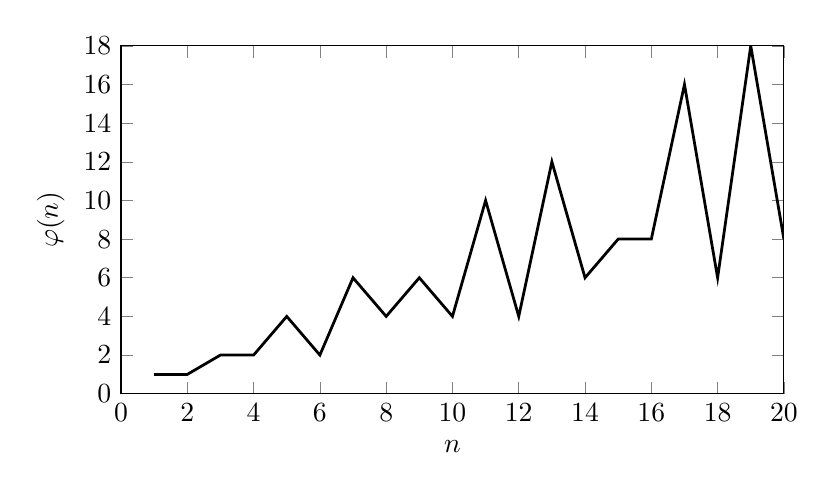
\begin{tikzpicture}
			\begin{axis}
				[
				xlabel={$n$}, ylabel={$\varphi(n)$}, xmin=0, xmax=20,
				ymin=0, ymax=18,
				height=6cm,
				width=10cm,
				xtick={0,2,4,6,8,10,12,14,16,18,20},
				ytick={0,2,4,6,8,10,12,14,16,18},
				]
				
				\addplot[line width=1pt]
				coordinates{
					(1,1) (2,1) (3,2) (4,2) (5,4) (6,2) (7,6) (8,4) (9,6) (10,4) (11,10) (12,4) (13,12) (14,6) (15,8) (16,8) (17,16) (18,6) (19,18) (20,8)};
			\end{axis}
		\end{tikzpicture}
		\item Sei $p$ eine Primzahl. Dann ist $\varphi(p) = p-1$.
		\item Sei $k \geq 1$ und $p$ prim. Dann gilt
			\begin{align*}
				\varphi(p^k) &= p^k - \left|\left\{0 < a \leq p^k \mid \ggt\left(a,p^k\right)>1\right\}\right|\\
				&= p^k - p^{k-1}
			\end{align*}
			Eine Beobachtung:
			\begin{align*}
				\varphi(1) + \varphi(p) + \varphi(p^2) + \dots + \varphi(p^k) &= 1 + (p-1) + (p^2-p) + \dots + (p^k-k^{k-1}) \\
				&= p^k
			\end{align*}
	\end{enumerate}
\end{exmp*}

\begin{thm}\autolabel
	Sei $n \in \Z$. Dann gilt
	\[ \sum_{d \mid n} \varphi(d) = n. \]
\end{thm}

Nun wollen wir uns mit der Berechnung der Eulerschen $\varphi$-Funktion beschäftigen. Für Primzahlpotenzen haben wir das schon getan und wollen dies jetzt auf allgemeine natürliche Zahlen anhand ihrer Primfaktorzerlegung fortsetzen.

\begin{thm}\autolabel\video
	$\varphi$ ist eine multiplikative Funktion, d.h. für $m,n \in \N$ mit $\ggt(m,n) = 1$ gilt $$\varphi(mn) = \varphi(m)\varphi(n).$$
\end{thm}

\begin{cor}
	Sei $m = p_1^{k_1} p_2^{k_2} \dotsm p_r^{k_r}$ mit $p_1 < p_1 < \dots < p_r$ Primzahlen und $k_i \geq 0$ für $1 \leq i \leq r$. Dann gilt
	\begin{align*}
		\varphi(m) &= \prod_{i=1}^r \left( p_i^{k_1} - p_i^{k_i-1} \right)\\
		\noalign{\centering oder}
		\varphi(m) &= m \cdot \prod_{\substack{p \mid  m \\ p \ \text{prim}}} \left( 1-\frac{1}{p} \right).
	\end{align*}
\end{cor}
\lecturefilevideo{23.04.2021}{Kleiner Satz von Fermat}
\begin{thm}[Fermats kleiner Satz]\autolabel
	Sei $a \in \Z,\ p $ eine Primzahl. Dann gilt
	\[ a^p \equiv a \mod p. \]
	Ist $p \nmid a$, dann gilt
	\[ a^{p-1} \equiv 1 \mod p. \]
\end{thm}

\begin{thm}[Euler]\autolabel
	Sei $M \geq 2,\ a \in \Z$ mit $\ggt(a,M) = 1$. Dann gilt
	\[ a^{\phi(M)} \equiv 1 \mod M. \]
\end{thm}

\begin{rem*}
	$(\Z/M\Z)^*$ ist eine Gruppe der Ordnung $\phi(M)$. Ist $a \in (\Z/M\Z)^*$, dann gilt $a^{\phi(M)} ) 1$ in $(\Z/M\Z)^*$.
\end{rem*}

\section{Ordnungen}\filevideo{Ordnungen}

Sei $M \in \Z_{\geq 2},\ a \in \Z$ mit $\ggt(a,M)=1$. Wir wissen bereits 
\[ a^{\phi(M)} \equiv 1 \mod M. \]
Sei $E = \{k \in \N \mid a^k \equiv 1 \bmod M\}$. Dann ist $E \neq \emptyset$.

\begin{defn*}[Ordnung]\index{Ordnung}
	Das kleinste Element in $E$ nennen wir die \emph{Ordnung von $\emph{a}$ modulo $\emph{M}$}.
	\begin{notat*}
		$\ord_M(a)$
	\end{notat*}
\end{defn*}

\begin{exmp*}
	Seien $M = 5,\ a= 2$. Für welche $k \in \N$ gilt $2^k \equiv 1 \bmod 5$?
	\[ 2^1 \equiv 2,\ 2^2 \equiv 4,\ 2^3 \equiv 3,\ 2^4 \equiv 4 \mod 5 \]
	Also gilt $\ord_5 2 = 4$.
\end{exmp*}

\begin{lem}\autolabel
	Sei $M \in \Z_{\geq 2},\ a \in \Z$ mit $\ggt(M,a)=1$. Angenommen $a^k \equiv 1 \bmod M$. Dann gilt
	\[ \ord_M a \mid k. \]
\end{lem}

\video Wir betrachten zunächst eine Verschärfung des Satzes von Euler (\ref{4.5}):\\
Sei $M \in \Z_{\geq 2}$ von der Form
\[ M = p_1^{k_1} \dotsm p_r^{k_r} \]
mit $p_1 < \dots < p_r$ prim und $k_1, \dotsc, k_r \geq 1$. Setze
\[ \lambda(M) = \kgv_{1 \leq i \leq r} \left( p_1^{k_i} - p_i^{k_i - 1} \right) = \kgv_{1 \leq i \leq r} \phi\left(p_i^{k_i}\right) \]
Vergleiche mit
\[ \phi(M) = \prod_{i=1}^r \left( p_1^{k_i} - p_i^{k_i - 1} \right) \]
Unser Ziel ist nun, zu zeigen, dass wir im Satz von Euler $\phi(M)$ einfach durch $\lambda(M)$ ersetzen können, was kleiner als $\phi(M)$ sein kann.

\begin{thm}\autolabel
	Sei $M \in \Z_{\geq 2}$ wie oben, d.h.
	\[ M = p_1^{k_1} \dotsm p_r^{k_r} \]
	mit $p_1 < \dots < p_r$ prim und $k_1, \dotsc, k_r \geq 1$. Sei $a \in \Z$ mit $\ggt(a,M)=1$. Dann gilt
	\[ a^{\lambda(M)} \equiv 1 \mod M. \]
\end{thm}

\begin{defn*}[Primitivwurzel]\index{Primitivwurzel}
	Sei $M \geq 2$. Eine ganze Zahl $g \in \Z$ mit $\ggt(M,g)=1$ und 
	\[ \left\{ \bar{g}, \bar{g}^2,\dotsc, \bar{g}^{\phi(M)} \right\} = (\Z/M\Z)^* \]
	nennen wir \emph{Primitivwurzel modulo $\emph{M}$}.
\end{defn*}

\begin{exmp*}
	\begin{enumerate}
		\item 2 ist eine Primitivwurzel modulo 5, denn
		\[ \left\{2,2^2,2^3,2^4 \right\} = (\Z/M\Z)^*. \]
		\item Gibt es eine Primitivwurzel modulo $M=15$? In anderen Worten, gibt es $g \in \Z$, $\ggt(g,15)=1$, mit $\left\{ g,g^2,\dotsc,g^{\phi(15)} \right\} = (\Z/15\Z)^*$?\\
			Bemerke $\phi(15) = \phi(5)\phi(3) = 4 \cdot 2 = 8$, aber $\lambda(15) = \kgv(\phi(15),\phi(3)) = 4$.\\
			Also für $\ggt(g,15) = 1$ $\left|\left\{ g,g^2,\dotsc, g^{\phi(15)} \right\}\right| \leq 4$, denn $g^{\lambda(15)} = g^4 \equiv 1 \bmod 15$. Also gibt es keine Primitivwurzel modulo 15.
		\item Sei $M = pq$ mit $pq,$ prim, $p,q > 2$. Dann ist $\phi(M) = (p-1)(q-1)$, aber $\lambda(M) = \kgv(p-1,q-1) < \phi(M)$. Also gibt es keine Primitivwurzel modulo $M$.
	\end{enumerate}
\end{exmp*}

Im Weiteren wollen wir nun zeigen, dass es im Allgemeinen zu jeder Primzahl auch eine Primitivwurzel gibt. Dafür benötigen wir zunächst folgende Lemmata:

\begin{lem}\filevideo{Primitivwurzeln}\autolabel
	Seien $a,b \in (\Z/M\Z)^*$ mit $M \in \Z_{\geq 2}$, $A = \ord_M a, B = \ord_M b$. Angenommen $\ggt(A,B)=1$, dann gilt
	\[ \ord_M ab = AB. \]
\end{lem}

\begin{lem}\autolabel
	Seien $a_1,\dotsc,a_m \in (\Z/M\Z)^*$ mit $M \in \Z_{\geq 2}$ und $A = \kgv(\ord_M(a_1),\dotsc, \ord_M(a_m))$. Dann $\existss b \in (\Z/M\Z)^*$ mit $\ord_M b = A$.
\end{lem}

\section{Primitivwurzeln}\video

\begin{thm}\autolabel
	Sei $p$ eine Primzahl. Dann gibt es eine Primitivwurzel modulo $p$.
\end{thm}

Das bedeutet, dass es $g \in \Z$ (oder $g \in \N$) gibt mit $\left\{ g,g^2,\dotsc,g^{p-1} \right\} = (\Z/p\Z)^*$. Wie klein kann man dieses $g$ nun wählen?

\begin{conj*}
	Sei $p$ eine Primzahl. Dann gibt es eine Primitivwurzel $g \in \N$ mit $g < 2 (\log p)^2$.
\end{conj*}

Von einem Beweis dieser Vermutung sind wir noch sehr weit enfernt. Doch was ist bisher bekannt? Es gib eine Primitivwurzel $g \in \N$ modulo $p$ mit $g < Cp^{\frac{1}{4} + \epsilon}$, wobei $C,\epsilon>0$ und $\epsilon$ beliebig klein. Dieses Resultat folgt aus Arbeiten von D.A. Burgess aus dem Jahre 1962.

\begin{conj*}[Artin]
	2 ist eine Primitivwurzel für unendlich viele Primzahlen $p$.
\end{conj*}

Eine leicht abgeänderte und "aufgefächerte" Variante dieser Vermutung stellt der folgende Satz dar, der sich auch tatsächlich beweisen ließ:

\begin{thm*}[Heath-Brown, 1986]
	Mindestens eine der Zahlen 2,3,5 ist eine Primitivwurzel für unendlich viele Primzahlen $p$.
\end{thm*}
Um den Satz \ref{4.10} nun beweisen zu können bedarf es noch ein wenig Vorbereitung:\lecturevideo{27.04.2021}

\begin{thm}\autolabel
	Sei $P(X) = a_nX^n + \dots + a_1X + a_0$ mit $a_n,\dotsc,a_0 \in \Z$ und $p$ prim. Angenommen $p \nmid a_n$, dann hat die Gleichung $P(X) \equiv 0 \bmod p$ höchstens $n$ verschiedene Lösungen modulo $p$.
\end{thm}

Für welche $M \in \N_{\geq 2}$ gibt es eine Primitivwurzel modulo $M$?\video

\begin{thm}\autolabel
	Sei $k \in \N$ und $p > 2$ eine Primzahl. Dann gibt es eine Primitivwurzel modulo $p^k$.
\end{thm}

\begin{lem}\autolabel
	Sei $p$ eine ungerade Primzahl und $k \in \N$. Dann gilt
	\[ (1+p)^{p^{k-1}} \equiv 1+p^k \mod p^{k+1}. \]
\end{lem}
	\chapter{Primzahltests}\filevideo{Primzahltests}

Wir machen nun einen kleinen Ausflug, um die Theorien von Ordnungen und Kongruenzrechnung zu verwenden und uns über Primzahltests zu unterhalten. Eine große Frage hierbei ist, wie man für eine natürliche Zahl $n \in \N$ möglichst schnell herausfinden kann, ob sie eine Primzahl ist oder nicht.\footnote{Dieses Kapitel ist nicht klausurrelevant.}

Komplexität eines Algorithmus':\\
$L = $ Zahl der Bits, die für den Input notwendig sind

\begin{exmp*}
	Um eine natürliche Zahl $N$ zu beschreiben benötigt man $\sim\log_{10}N$ Ziffern im Dezimal oder $\sim\log_2N$ Bits.
\end{exmp*}

Wir nennen einen Algorithmus polynomiell, wenn seine Laufzeit begrenzt ist durch $c2^a$ mit $c,a > 0$.

\begin{exmp*}
	\begin{enumerate}[label={\roman*})]
		\item Der Euklidische Algorithmus angewandt auf $M,N \in \N$ mit $M<N$ benötigt $\sim c\log_{10}N$ Schritte. Dies ist ein polynomieller Algorithmus.
		\item Um eine Primfaktorzerlegung von $N \in \N$ naiv herzuleiten indem man alle Teiler $\leq \sqrt{N}$ probiert, benötigt man $\sim \sqrt{N} = e^{\frac{\log N}{2}} \cong e^{c2}$ Schritte. Dies nennen wir einen exponentiellen Algorithmus.
 	\end{enumerate}
\end{exmp*}

Die schnellste Laufzeit für eine Primfaktorzerlegung ist in $\sim c_1 e^{c_2\sqrt[3]{\log N \log\log N}}$ Schritten möglich mit $c_1,c_2 > 0$.

\begin{frage*}
	Wie kann man schnell testen, ob eine natürliche Zahl $N \in \N$ prim ist?
\end{frage*}

Fermats kleiner Satz (\ref{4.4}) besagt, dass für $N \in \N, a \in \Z, N \nmid a, N$ prim, $A^{N-1} \equiv 1 \bmod N$ gilt. (Achtung: Die Rückrichtung gilt hierbei im Allgemeinen nicht!) 

\begin{defn*}
	Eine natürliche Zahl $N$ mit $a^{N-1} \equiv 1 \bmod N$ für alle $a \in \Z$ mit $\ggt(a,N)=1$ nennen wir eine Carmichael Zahl\footnote{Nach Robert Daniel Carmichael (1879-1967), US-amerikanischer Mathematiker}.
\end{defn*}

\begin{thm*}[Alford\protect\footnotemark, Granville\protect\footnotemark, Pomerance\protect\footnotemark, 1951]
	\footnotetext{William Robert Alford (1937-2003), ein US-amerikanischer Mathematiker}
	\footnotetext{Andrew James Granville (geb. 1962), ein britisch-kanadischer Mathematiker}
	\footnotetext{Carl Bernard Pomerance (geb. 1944), ein US-amerikanischer Mathematiker}
	Es gibt unendlich viele Carmichael Zahlen.
\end{thm*}

\begin{frage*}
	Weitere Eigenschaften von Primzahlen?
\end{frage*}

\begin{thm}[Rabin\protect\footnotemark]\autolabel\video
	\footnotetext{Nach Michael O. Rabin (geb. 1931), ein israelischer Informatiker}
	Sei $N$ ungerade, $a \in \Z$, $N \nmid a$. Angenommen $N-1 = 2^k \cdot m$ mit $m$ ungerade. Ist $N$ prim, dann gilt
	\[ a^m \equiv 1 \mod N \]
	oder es gilt $0 \leq j \leq k-1$ mit 
	\[ a^{2^jm} \equiv -1 \mod N. \]
\end{thm}

\begin{thm*}
	Sei $N$ ungerade, $a \in \Z$, $N \nmid a$ und $N-1 = 2^km$ mit $m$ ungerade. Ist $a^m \not\equiv 1 \bmod N$ und $a^{2^jm} \not\equiv -1 \bmod N$ für alle $0 \leq j \leq k-1$, dann ist $N$ zusammengesetzt.
\end{thm*}

\begin{defn*}
	In diesem Fall nennen wir $a$ einen Zeugen für die Zusammengesetztheit von $N$.
\end{defn*}

\begin{thm*}
	Sei $N$ ungerade und zusammengesetzt, Dann sind mindestens 75\% der Zahlen $1,2,\dotsc,N-1$ Zeugen für die Zusammengesetztheit von $N$.
\end{thm*}

\begin{idee*}
	Führe den Rabin-Test mit $k$ zufällig gewählten Zahlen $a$ aus. Ist $N$ zusammengesetzt, dann ist die Wahrscheinlichkeit, dass wir einen Zeugen nach $k$ Schritten finden \( \geq 1 - \left( \frac{1}{4} \right)^k \)
\end{idee*}

\begin{rem*}
	Wenn die verallgemeinerte Riemann-Hypothese gilt, dann gibt es für zusammengesetzte $N$ einen Zeugen $a < 2(\log N)^2$. Dies führt zu einem polynomiellen Algorithmus, der die Zusammengesetztheit von $N$ erkennt.
\end{rem*}

\section{Die Pollard'sche $\rho$-Methode}\filevideo{Pollard-$\rho$-Methode}
\footnote{Nach John M. Pollard (geb. 1941), ein britischer Mathematiker}

Angenommen $N \in \N$ ist zusammengesetzt. Unser Ziel ist, einen echten Teiler von $N$ zu finden.

Sei $b \in \Z$ und betrachte die Folge $x_0,x_1,x_2,\dotsc$ von Restklassen modulo $N$, definiert auch $x_0 = 1, x_{i+1} \equiv x_i^2+b \bmod N$ für $i \geq 0$.

Sei $\nu(m)$ für $m \in \N$ die größte Potenz von 2, die kleiner als $m$ ist.

\begin{exmp*}
	\( \nu(5)=4, \nu(8)=4,\nu(12)=8 \)
\end{exmp*}

Wir berechnen $\ggt(x_i-x_{nu(i)}, N)$. Unsere Erwartung ist, dass wenn wir das für $i < 4,5 N^{\frac{1}{4}}$ tun die Wahrscheinlichkeit, dass wir einen echten Teiler von $N$ gefunden haben, $> \frac{1}{2}$ ist.

Hemiasdb Sei $p \leq \sqrt{N}$ ein Primteiler von $N$ und $q = \lfloor\sqrt{2p}\rfloor + 1$. Betrachte $x_0,x_1,\dotsc,x_q$ modulo $q$.

\emph{1. Ziel:} Finde $0 \leq k, l \leq q$ mit $x_k-x_l \equiv  0 \bmod p$.

Die Wahrscheinlichkeit, dass alle $x_0,x_1,\dotsc,x_q$ modulo $p$ verschieden sind ist $\left( 1-\frac{1}{p} \right) \cdot \left( 1-\frac{2}{p} \right) \dotsm \left( 1-\frac{q}{p} \right)$. Wie groß ist das?
\begin{align*}
	\log \left( 1-\frac{1}{p} \right) \cdot \left( 1-\frac{2}{p} \right) \dotsm \left( 1-\frac{q}{p} \right) &= \sum_{r=1}^q \log \left( 1 - \frac{r}{q} \right)\\
	&\leq - \sum_{r=1}^q \frac{r}{p} = -\frac{1}{2} \frac{q(q+1)}{p}\\
	&< -1
\end{align*}
Die Wahrscheinlichkeit, dass $x_0,x_1,\dotsc,x_q$ modulo $p$ paarweise verschieden sind, ist also $< e^{-1}<\frac{1}{2}$

\begin{rem*}
	$q < \sqrt{2\sqrt{N}} + 2 < 1,5 N^{\frac{1}{4}}$
\end{rem*}

Unser Problem ist nun, dass wir gerne $\ggt(x_k-x_l,N)$ für alle $0\leq k, l \leq q$ berechnen würden, dies wären jedoch $\sim N^{\frac{1}{4}} \cdot N^{\frac{1}{4}} \sim N^{\frac{1}{2}}$ Berechnungen!

\begin{idee*}
	Ist 
	\begin{align*}
		x_k &\equiv x_l \mod p, \\
		\noalign{so auch}
		x_{k+1} &\equiv x_{l+1} \mod p\\
		x_{k+2} &\equiv x_{l+2} \mod p\\
		\noalign{\centering $\vdots$}
	\end{align*}
	Angenommen, wir haben $l < k$ mit $x_k \equiv x_l \bmod p$ und $0 \leq l, k \leq q$. Wähle $m \in \N$ mit 
	\[ 2^{m-1} < \max\{l,k-l\} \leq 2^m. \]
	Dann gilt
	\[ x_{k-l} \equiv x_{2^m} \mod p \]
	und 
	\begin{align*}
		k-l + 2^m &< k-l + 2\max\{l,k-l\}\\
		&\leq 4,5 N^{\frac{1}{4}}
	\end{align*}
\end{idee*}
	\chapter{Quadratreste}\lecturefilevideo{30.04.2021}{Quadratreste, Teil 1}

Bisher haben wir lineare Kongruenzgleichungen 
\[ ax+b \equiv 0 \mod M \]
mit $a,b \in \Z,\ M \in \N$ betrachtet. Nun wollen wir uns die Frage stellen, was passiert, wenn wir zu quadratische Kongruenzgleichungen übergehen.

Seien $a,b,c \in \Z,\ M \in \N_{\geq 2}$. Wann hat die Gleichung
\[ ax^2 + bx + c \equiv 0 \mod M \]
eine Lösung? Laut dem chinesischen Restsatz genügt es, $M= p^k$ mit $p$ prim zu betrachten. Wir beginnen mit dem einfachsten Fall
\[ x^2 \equiv a \mod p \]

\begin{defn*}[quadratischer (Nicht-)Rest] \index{quadratischer (Nicht-)Rest}
	Sei $a \in \Z,\ p$ prim mit $p \nmid a$. Dann nennen wir $a$ einen \emph{quadratischen Rest/Nichtrest} modulo $p$, falls $x^2 \equiv a \bmod p$ lösbar ist/keine Lösung hat.
\end{defn*}

\begin{exmp*}
	\begin{itemize}
		\item[$p=7$:] Quadratische Reste: 1,2 ,4\\
		Quadratische Nichtreste: 3,5,6
		\item[$p=5$:] Quadratische Reste: 1,4\\
		Quadratische Nichtreste: 2,3
	\end{itemize}
\end{exmp*}

\begin{thm}\autolabel
	Sei $p$ eine ungerade Primzahl. Dann gibt es $\frac{p-1}{2}$ quadratische Reste und $\frac{p-1}{2}$ quadratische Nichtreste modulo $p$.
\end{thm}
\pagebreak
\begin{defn*}[Legendre\protect\footnotemark{} Symbol]\index{Legendre Symbol}
	\footnotetext{Nach Adrien-Marie Legendre (1752-1833), ein französischer Mathematiker}
	Sei $p$ eine ungerade Primzahl und $a \in \Z$. Wir definieren das \emph{Legendre Symbol} als\video
	\[ \left( \frac{a}{p} \right) = \begin{cases}
		1 \qquad &\text{falls $a \equiv x^2 \bmod p$ eine Lösung hat}\\
		-1 \qquad &\text{falls $a$ ein quadratischer Nichtrest modulo $p$ ist}\\
		0 \qquad &p \mid a
	\end{cases} \]
\end{defn*}

\begin{exmp*}
	Sei $p=7$:\\
	\( \left( \frac{1}{7} \right) = \left( \frac{2}{7} \right) = \left( \frac{4}{7} \right) = 1 \)\\
	\( \left( \frac{7}{7} \right) = 0 \)\\
	\( \left( \frac{3}{7} \right) = \left( \frac{5}{7} \right) = \left( \frac{1}{6} \right) = -1 \)
\end{exmp*}

\begin{thm}\autolabel
	Sei $p$ eine ungerade Primzahl, $a,b\in \Z$. Dann gilt
	\[ \left( \frac{ab}{p} \right) = \left( \frac{a}{p} \right) \left( \frac{b}{p} \right) \]
\end{thm}

\begin{frage*}\filevideo{Quadratreste, Teil 2}
	Wie lassen sich die Legendre Symbole berechnen?
\end{frage*}

\begin{thm}[Euler]\autolabel
	Sei $p$ eine ungerade Primzahl, $a \in \Z$ mit $p \nmid a$. Dann gilt
	\[ \left( \frac{a}{p} \right) \equiv a^{\frac{p-1}{2}} \mod p. \]
\end{thm}

\begin{cor}\autolabel
	Sei $p$ eine ungerade Primzahl. Dann gilt
	\[ \left( \frac{-1}{p} \right) = \begin{cases}
		1 \qquad &\text{für $p \equiv 1 \bmod 4$}\\
		-1 \qquad &\text{für $p \equiv -1 \bmod 4$}
	\end{cases} \]
\end{cor}

\begin{thm}[Quadratische Reziprozität]\autolabel
	Seien $p,q$ ungerade Primzahlen mit $p \neq q$. Dann gilt\filevideo{Quadratreste, Teil 3}
	\[ \left( \frac{p}{q} \right) \left( \frac{q}{p} \right) = (-1)^{\frac{(p-1)(q-1)}{4}}. \]
\end{thm}

\begin{thm}\autolabel
	Sei $p$ eine ungerade Primzahl. Dann gilt
	\[ \left( \frac{2}{p} \right) = (-1)^{\frac{p^2-1}{8}} = \begin{cases}
		1 \quad &p \equiv \pm 1 \bmod 8\\
		-1 \quad &p \equiv \pm 3 \bmod 8
	\end{cases} \]
\end{thm}

\begin{exmp*}
	\begin{align*}
		\left( \frac{-70}{11} \right) &= \left( \frac{5}{11} \right) \left( \frac{7}{11} \right) \left( \frac{-1}{11} \right) \left( \frac{2}{11} \right)\\
		&= \left( \frac{11}{5} \right) (-1) \left( \frac{11}{7} \right) (-1)(-1)\\
		&= \left( \frac{1}{5} \right) (-1) \left( \frac{4}{7} \right)\\
		&= -1
	\end{align*}
\end{exmp*}

\begin{exmp*}
	Bestimme $\left(\frac{3}{p}\right)$ für ungerade Primzahlen $p \neq 3$.
	
	\emph{Fall 1:} $p \equiv 1 \bmod 4$. Dann gilt
	\[ \left(\frac{3}{p}\right) = \left(\frac{p}{3}\right) \]
	und $\left(\frac{3}{p}\right) = 1 \iff p \equiv 1 \bmod 3$.
	
	\emph{Fall 2:} $p \equiv -1 \bmod 4$. Dann gilt
	\[ \left(\frac{3}{p}\right) = -\left(\frac{p}{3}\right) \]
	und $\left(\frac{3}{p}\right) = 1 \iff p \equiv 2 \bmod 3$.
	
	Insgesamt folgt also
	\[ \left(\frac{3}{p}\right) = \begin{cases}
		1 \qquad & p \equiv \pm 1 \mod 12\\
		-1 \qquad & p \equiv \pm 5 \mod 12
	\end{cases} \]
\end{exmp*}

\begin{thm}\autolabel
	Es gibt unendlich viele Primzahlen $p \equiv 1 \bmod 4$.
\end{thm}

\begin{obs*}
	Das Legendre Symbol $\left(\frac{a}{p}\right)$ ist beinahe periodisch in $p$.\video
\end{obs*} 

\begin{thm}\autolabel
	Sei $a \in \Z\setminus\{0\},\ p,q $ ungerade Primzahlen mit $p \nmid a$ und $q \nmid a$. Angenommen $a \equiv 1 \bmod 4$ und $p \equiv q \bmod |a|$, oder $a \not\equiv 1 \bmod 4$ und $p \equiv q \bmod 4|a|$, dann gilt
	\[ \left(\frac{a}{p}\right) = \left(\frac{a}{q}\right) \]
\end{thm}

\begin{lem}\autolabel
	Seien $u_1,\dotsc,u_r \in \Z$ ungerade. Dann gilt
	\[ \sum_{i=1}^r \frac{u_i -1}{2} \equiv \frac{u_1 \dotsm u_r - 1}{2} \mod 2 \]
	und
	\[ \sum_{i=1}^r \frac{u_i^2 -1}{8} \equiv \frac{(u_1\dotsm u_r)^2-1}{8} \mod 2 \]
\end{lem}


	\chapter{Summen von Quadraten}\lecture{11.05.2021}

\section{Summen von zwei Quadraten}

Die Frage, mit der wir uns in diesem Kapitel beschäftigen wollen, ist welche natürlichen Zahlen wir als Summe von zwei Quadraten schreiben können.

\begin{exmp*}
	\( 5 = 1^2+2^2 \)\\
	\( 3 = \square + \square \)? $\implies$ keine Lösung\\
	\( 2 = 1^2 +1^2 \)\\
	\( 4 = 2^2 + 0^2 \)
\end{exmp*}

\begin{lem}\autolabel
	Seien $a,b \in \Z$, $p$ eine ungerade Primzahl mit $p \nmid ab$ und $p \mid a^2 + b^2$. Dann gilt
	\[ p \equiv 1 \mod 4. \]
\end{lem}

\begin{cor*}
	Ist $p \geq 3$ prim, $p = a^2+b^2$ mit $a,b \in \Z$, dann gilt $p \equiv 1 \bmod 4$.
\end{cor*}

\begin{thm}[Fermat]\autolabel
	Sei $p$ eine Primzahl mit $p \equiv 1 \bmod 4$. Dann gibt es $a,b \in \Z$ mit $p = a^2+b^2$.
\end{thm}

\begin{lem}\autolabel
	Angenommen $m,n \in \Z$ mit $m = a^2+b^2$ und $n = c^2 + d^2$ für gewisse $a,b,c,d \in \Z$. Dann ist auch $m \cdot n$ die Summe von zwei ganzzahligen Quadraten.
\end{lem}

Wie können wir nun alle $n \in \N$ finden, die wir als Summe von zwei Quadraten schreiben können?

\begin{cor}\autolabel
	Sei $n \in \N$. Dann gilt $n = a^2+b^2$ für $a,b \in \Z$ genau dann, wenn $n$ die Form
	\[ n = 2^k m^2 p_1 \dotsm p_r \]
	mit $k \geq 0$, $m \in \Z$, $p_1, \dotsc,p_r$ Primzahlen mit $p_i \equiv 1 \bmod 4$ hat.
\end{cor}

\begin{thm}[Verschärfung von Satz \ref{7.2}]\autolabel
	Sei $n \in \N$ und definiere
	\[ r_2(n) = \left| \left\{ (x,y) \in \Z^2 \mid n = x^2 + y^2 \right\} \right|. \]
	\begin{enumerate}[label={\roman*})]
		\item $\frac{r_2(n)}{4}$ ist eine multiplikative Funktion.
		\item Sei $p$ prim und $k \in \N$. Dann gilt
			\[ \frac{r_2(p^k)}{4} = \begin{cases}
				k+1 \quad &\text{für } p \equiv 1 \bmod 4\\
				0 \quad &\text{für } p \equiv 3 \bmod 4 \ \text{und $k$ ungerade}\\
				1 \quad &\text{für } p \equiv 4 \bmod 4 \ \text{und $k$ gerade}\\
				1 \quad &\text{für } p = 2
			\end{cases} \]
	\end{enumerate}
\end{thm}

\begin{exmp*}
	$p \equiv 3 \bmod 4 \quad \checkmark$\\
	$p = 2, 2 = (\pm 1)^2 + (\pm 1)^2$\\
	Ist $p \equiv 1 \bmod 4$ mit $p = a^2+b^2$, dann sind auch $(\pm a,\pm b),(\pm b, \pm a)$ Lösungen.
\end{exmp*}

\begin{thm}[Dirichlet]\autolabel
	Sei $n \in \N$. Dann gilt
	\[ r_2(n) = 4 \sum_{\substack{d \mid n \\ d \equiv 1 \bmod 2}} (-1)^{\frac{d-1}{2}} \]
\end{thm}

\section{Summen von vier Quadraten}

\begin{frage*}
	Angenommen, wir wollen \emph{jedes} $n \in \N$ schreiben als
	\[ n = \square + \square + \square + \square + \square + \square + \dots \]
	Wie viele Quadrate benötigt man mindestens?
\end{frage*}

\emph{Beobachtung:} 4 Quadrate sind ausreichend.

\begin{thm}[Lagrange\protect\footnotemark{} 1770]\autolabel
	\footnotetext{Nach Joseph-Louis Lagrange (1736-1813), ein italienischer Mathematiker und Astronom}
	Jede natürliche Zahl $n$ kann als Summe vn vier ganzzahligen Quadraten geschrieben werden.
\end{thm}

\begin{lem}\autolabel
	Ist $m = \square + \square + \square + \square$ und $n = \square + \square + \square + \square$, dann gilt auch
	\[ mn = \square + \square + \square + \square. \]
\end{lem}

Mit diesem Lemma können wir uns als Ziel setzen, jede beliebige Primzahl $p$ als Summe von maximal vier Quadraten zu schreiben.

\begin{lem}\autolabel
	Sei $p>2$ prim. Dann gibt es $m \in \N$ mit $m<p$ und 
	\[ mp = \square + \square + \square + \square. \]
\end{lem}
\section{Summen von drei Quadraten}\lecture{14.05.2021}

\begin{frage*}
	Für welche $n \in \N$ genügen uns sogar schon 3 Quadrate?
\end{frage*}

Erste Beobachtung: $\square \equiv 0,1,4 \bmod 8$.
\begin{itemize}
	\item Ist $n \in \N$ mit $n \equiv 7 \bmod 8$, dann $n \neq \square + \square + \square$
	\item Angenommen $n \in \N$ mit $n = a^2+b^2+c^2$ mit $a,b,c \in \Z$ und $4 \mid n$. Dann haben wir
	\[ 0 \equiv n \equiv a^2+b^2+c^2 \bmod 4. \]
	Daraus folgt $2 \mid a$, $2\mid b$, $2 \mid c$, also
	\[ \frac{n}{4} = \left(\frac{a}{2}\right)^2 + \left(\frac{b}{2}\right)^2 + \left(\frac{c}{2}\right)^2 \]
\end{itemize}
Folgerung: Ist $n = (8k+7) \cdot 4^l$ mit $k \in \Z_{\geq 0}$, $l \in \Z_{\geq 0}$, dann ist $n \neq \square + \square + \square$.\pagebreak

\begin{thm}[Gauß\protect\footnotemark]\autolabel
	\footnotetext{Nach Carl Friedrich Gauß (1777-1855), ein deutscher Mathematiker, Statistiker, Astronom, Geodät und Physiker}
	Jedes $n \in \N$, das nicht die Form $n = 4^l(8k+7)$ mit $k,l \in \Z_{\geq 0}$ hat, kann als Summe von drei Quadraten geschrieben werden.
\end{thm}

Eine Anwendung: Dreieckszahlen, also Zahlen der Form
\[ a_n = \frac{n(n+1)}{2}. \]

\begin{cor}\autolabel
	Jede natürliche Zahl $n \in \N$ kann als Summe von drei Dreieckszahlen geschrieben werden, das heißt $n = \triangle + \triangle + \triangle $.
\end{cor}

Allgemeiner: Sei $F(x_1,\dotsc,x_k) \in \Z[x_1,\dotsc,x_k]$ ein homogenes Polynom von Grad 2, z.B. $x_1^2 + x_3x_4 + x_2^2 + \dots$

\begin{frage*}
	Wann kann man jede natürliche Zahl schreiben als $n = F(x_1,\dotsc,x_k)$ mit $x_1,\dotsc,x_k \in \Z$?
\end{frage*}

Um diese Frage beantworten zu können benötigen wir zunächst etwas Terminologie:
\begin{itemize}
	\item Wir nennen $F$ \emph{positiv definit}, falls $F(x_1,\dotsc,x_k) > 0$ für alle \( (x_1,\dotsc,x_k) \in \R^k \setminus \{0\} \).
	\item Wir nennen $F$ \emph{gerade}, falls jeder Koeffizient von $x_ix_j$ mit $i \neq j$ gerade ist.
\end{itemize}

\begin{thm*}[15-Satz von Conway\protect\footnotemark{} und Schneeberger\protect\footnotemark, 1993]
	\footnotetext{John Horton Conway (1937-2020), ein britischer Mathematiker}
	\footnotetext{William Allan Schneeberger (geb. 1970), Promotionsstudent Conways}
	Sei $F(x_1,\dotsc,x_k)$ eine gerade positiv definite quadratische Form mit ganzen Koeffizienten. Falls $F$ die Zahlen $n = 1,\dotsc, 15$ darstellt, dann stellt $F$ alle natürlichen Zahlen dar.
\end{thm*}

\begin{thm*}[290-Theorem von Bhargava\protect\footnotemark{} und Hanke\protect\footnotemark{}, 2005]
	\footnotetext{Manjul Bhargava (geb. 1974), ein kanadischer Mathematiker}
	\footnotetext{Jonathan Hanke, ein US-amerikanischer Mathematiker}
	Sei $F$ eine positiv definite quadratische Form mit ganzzahligen Koeffizienten. Falls $F$ die Zahlen $n=1, \dotsc, 290$ darstellt, dann stellt $F$ jede natürliche Zahl dar.
\end{thm*}

\section{Das Waringsche Problem}

\begin{thm*}[Jacobi]
	Jedes $n \in \N$ kann geschrieben werden als 
	\[ n = \square + \square + \square + \square. \]
\end{thm*}

\begin{frage*}
	Was passiert bei höheren Potenzen? Welche Zahlen können beispielsweise geschrieben werden als
	\[ n = a^3+b^3+c^3+d^3? \]
\end{frage*}

\begin{thm*}[Hilbert\protect\footnotemark]
	\footnotetext{Nach David Hilbert (1862-1943), ein deutscher Mathematiker}
	Sei $k \in \Z_{\geq 2}$. Dann gibt es eine natürliche Zahl $g(k)$, sodass jedes $n \in \N$ als Summe von höchstens $g(k)$ positiven $k$-ten Potenzen geschrieben werden kann. Das heißt für jedes $n \in \N$ gibt es $s \leq g(k),\ x_1,\dotsc,x_s \in \N$ mit $n = x_1^k + x_2^k + \dotsc + x_s^k$.
\end{thm*}

\begin{frage*}
	Was ist der kleinstmögliche Wert für $g(k)$?
\end{frage*}

\begin{defn*}
	Sei $g(k)$ die kleinstmögliche natürliche Zahl in Hilberts Satz.
\end{defn*}

\begin{exmp*}
	$g(2) = 4$ (Jacobi + Gauß)\\
	\( g(3) = 9 \)\\
	\( g(4) = 19 \)\\
	\( g(5) = 37 \)
\end{exmp*}

\begin{obs*}
	$g(k)$ wächst schnell in $k$, manchmal wegen kleinen Werten von $n$.
\end{obs*}

\begin{exmp*}
	Schreibe $2^k-1 = x_1^k + \dotsc + x_s^k$ mit $x_i \in \N$. Dann gilt $x_i = 1$ und $s = 2^k-1$. Es folgt $g(k) \geq 2^k-1$.
\end{exmp*}

\begin{idee*}
	Ist $k = 3$, dann kann jedes $n \in \N \setminus \{23,239\}$ als Summe von acht Kuben geschrieben werden.
\end{idee*}

\begin{defn*}
	Für $k \geq 2$ sei $G(k)$ die kleinste natürliche Zahl, sodass jedes hinreichend große $n \in \N$ als Summe von höchstens $G(k)$ positiven $k$-ten Potenzen geschrieben werden kann.
\end{defn*}

\emph{Bekannt:} $G(2) = 4,\ G(4) = 16,\ G(3) \leq 7$.

\begin{lem}\autolabel
	$G(3) \geq 4$
\end{lem}

\begin{thm*}[Wooley\protect\footnotemark{} 1992]
	\footnotetext{Nach Trevor Wooley (geb. 1964), ein britischer Mathematiker}
	Es gibt eine Konstante $C \in \R$ mit
	\[ G(k) \leq k \log k + k \log\log k + Ck. \]
\end{thm*}

\begin{lem*}
	\[ r_k(n) = \int_{0}^{1} T(\alpha)^s e^{-2\pi i \alpha n} \ d\alpha\]
\end{lem*}

\section{Quadratische Gleichungen in 2 Variablen über $\Q$}

Seien $a,b,c,d,e,f \in \Z$ und betrachte die Gleichung 
\[ Q(x,y) = ax^2+bxy+cy^2+dx+ey+f = 0 \]

\begin{exmp*}
	Hyperbel $x^2-y^2 = 1$\\
	Parabel $2x^2=y$\\
	Ellipsen $x^2+2y^2=3$\\
	Vereinigung von zwei Geraden $(x-2y+1)(2x-y)=0$
\end{exmp*}

Wir nennen $Q(x,y)$ \emph{reduzibel} über $\Q$ oder $\C$, falls $Q(x,y) = f(x,y)g(x,y)$ mit $\grad f \geq1$ und $\grad g \geq 1$ und $f,q \in \Q[x,y]$ oder $\C[x,y]$.

\begin{thm}\autolabel
	Seien $a,b,c,d,e,f \in \Z$. Falls $ ax^2+bxy+cy^2+dx+ey+f = 0$ eine rationale Lösung hat und über $\C$ irreduzibel ist, dann hat die Gleichung unendlich viele Lösungen.
\end{thm}

\begin{exmp*}
	\[ C: x^2+2y^2=3 \]
	hat den rationalen Punkt $(x_0,y_0) = (1,1)$. Berechne die Gerade $L$ durch $P = (x_0,y_0)$ mit Steigung $m \in \Q$.
	\[ L = \begin{cases}
		x = x_0 + t\\
		y = y_0 + t \cdot m
	\end{cases} \]
	Schnitt von $L$ und $C$:
	\begin{align*}
		(x_0+t)^2 + 2(y_0+tm)^2 &= 3\\
		(1+t)^2 + 2(1+tm)^2 &= 3\\
		\iff 2t + t^2 + 4tm + 2t^2m^2 &= 0\\
		t(t+2tm^2 + 2 + 4m) &= 0
	\end{align*}
	\begin{align*}
		\implies t &= 0 \ \text{oder}\\
		t &= -\frac{2+4m}{1+2m^2}
	\end{align*}
	$P'$ ist gegeben durch
	\begin{align*}
		x_1 &= 1- \frac{2+4m}{2+2m^2} = \frac{2m^2 - 4m - 1}{1+2m^2}\\
		y_1 &= 1-m \frac{2+4m}{1+2m^2}\\
		&= \frac{-2m^2 - 2m+1}{1+2m^2}
	\end{align*}
	Alle rationalen Lösungen von $x^2+2y^2 = 3$ können beschrieben werden durch
	\[ (x,y) = \left( \frac{2m^2-4m-1}{1+2m^2} , \frac{-2m^2 - 2m + 1}{1 + 2m^2} \right) \]
	für $m \in \Q$.
\end{exmp*}
	\chapter{Kettenbrüche}\lecture{18.05.2021}

\section{Endliche Kettenbrüche}

Zunächst: wir betrachten Kettenbrüche als Ausdrücke der Form
\[ b_0 + \frac{1}{b_1 + \frac{1}{b_2 + \dots + \frac{1}{b_n}}} \]
mit $b_0 \in \Z$, $b_1, \dotsc, b_n \in \N$. Als Kurzschreibweise benutzen wir die Notation
\[ \langle b_0,b_1,\dotsc,b_n \rangle. \]

\begin{rem*}
	Der Wert eines endlichen Kettenbruchs ist gleich einer rationalen Zahl.
\end{rem*}

\begin{lem}\autolabel
	Jede rationale Zahl kann als endlicher Kettenbruch geschrieben werden.
\end{lem}

\begin{cav*}
	Die Darstellung einer rationalen Zahl in der Form eines endlichen Kettenbruchs ist im allgemeinen nicht eindeutig:
	\[ \langle 0,1,1 \rangle = \frac{1}{1 + \frac{1}{1}} = \frac{1}{2} = \langle 0,2 \rangle \]
\end{cav*}

\begin{rem*}
	\begin{enumerate}[label={\roman*})]
		\item $a_m = \left\lfloor \frac{r_{m-1}}{r_m} \right\rfloor$ und \( \frac{r_{m+1}}{r_m} = \left\{ \frac{r_{m-1}}{r_m} \right\} = \frac{r_{m-1}}{r_m} - \left\lfloor \frac{r_{m-1}}{r_m} \right\rfloor. \)
		\item \( \frac{r_1}{r_2} = \langle a_2,a_3,\dotsc,a_k \rangle \) oder im Allgemeinen
		\[ \frac{r_{m-1}}{r_m} = \langle a_m, a_{m+1},\dotsc,a_k \rangle \]
	\end{enumerate}
\end{rem*}

\begin{exmp*}
	Wir wollen $\frac{137}{33}$ als Kettenbruch darstellen.
	\begin{align*}
		137 &= 4 \cdot 33 + 5 	& \frac{137}{33} &= 4 + \frac{5}{33}\\
		33 &= 6 \cdot 5 + 3 	& \frac{33}{5} 	&= 6 + \frac{3}{5}\\
		5 &= 1 \cdot 3 + 2 		& \frac{5}{3} 	&= 1 + \frac{2}{3}\\
		3 &= 1 \cdot 2 + 1 		& \frac{3}{2} 	&=1 + \frac{1}{2}
	\end{align*}
	Also ist \( \frac{137}{33} = \langle 4,6,1,1,2 \rangle \)
\end{exmp*}

\section{Unendliche Kettenbrüche}

Sei $\alpha \in \R \setminus \Q$. Unser Ziel ist es, $\alpha$ in der Form
\[ \alpha = \langle a_0,a_1,a_2,\dots\rangle \]
zu schreiben. Hierfür verwenden wir den Algorithmus aus Lemma \ref{8.1}:\\
Sei $\alpha_0 = \alpha$.
\[ a_0 = \lfloor \alpha_0 \rfloor,\ \alpha_1 = \frac{1}{\{\alpha_0\}}, \]
also 
\begin{align*}
	\alpha &= a_0 + \{\alpha_0\}\\
	&= a_0 + \frac{1}{\frac{1}{\{\alpha_0\}}}\\
	&= a_0 + \frac{1}{\alpha_1}
\end{align*}
\[ a_1 = \langle \alpha_1 \rangle,\ \alpha_2 = \frac{1}{\{ \alpha_1 \}} \implies \alpha_1 = a_1 + \frac{1}{\alpha_2} \]
\[ a_2 = \langle \alpha_2 \rangle,\ \alpha_3 = \frac{1}{\{ \alpha_2 \}} \]
\[\vdots\]
\[ a_n = \langle \alpha_n \rangle,\ \alpha_{n+1} = \frac{1}{\{ \alpha_n \}} \ \text{für } n \geq 0 \]

\begin{rem*}
	Es gilt für $i \geq 0$:
	\[ 0 < \{\alpha_i\} < 1 \]
	Also $\alpha_{i+1} = \frac{1}{\{\alpha_i\}} > 1$ und $a_{i+1} = \langle \alpha_{i+1} \rangle \in \N$.\\
	Nach $n$ Schritten
	\begin{align*}
		\alpha &= \langle a_0,a_1,a_2,\dotsc,a_{n-1},\alpha_n \rangle\\
		&= a_0 + \frac{1}{a_1 + \frac{1}{a_2 + \dots + \frac{1}{a_n}}}
	\end{align*}
\end{rem*}

\begin{rem*}
	Ist $\alpha \in \R \setminus \Q$, dann gilt $\alpha_n \neq 0 \ \foralll n \in \N$.
\end{rem*}

Ist $\alpha = \langle a_0,a_1,a_2,\dotsc,a_{n-1},\alpha_n \rangle$ wie oben, so nennen wir als Konvention die $a_i$ \emph{Elemente} des Kettenbruchs.

\begin{frage*}
	Warum würde man $\alpha \in \R \setminus \Q$ überhaupt als Kettenbruch schreiben wollen?
\end{frage*}

\begin{idee*}
	Die Elemente eines Kettenbruchs geben sehr gute Approximationen für die durch den Kettenbruch dargestellte Zahl.
\end{idee*}

\begin{defn*}[Teilbruch]\index{Teilbruch}
	Sei $\alpha \in \R \setminus \Q$, $\alpha = \langle a_0,a_1,a_2,\dotsc \rangle$. Dann nennen wir für $n \in \Z_{\geq0}$
	\[ \frac{p_n}{q_n} = \langle a_0,a_1,a_2,\dotsc,a_n \rangle \]
	den \emph{$\emph{n}$-ten Teilbruch} von $\alpha$.
\end{defn*}

\begin{exmp*}
	\begin{align*}
		\sqrt{2} &= \lfloor \sqrt{2}\rfloor + \{\sqrt{2}\}\\
		&= \lfloor \sqrt{2}\rfloor + \frac{1}{\frac{1}{\sqrt{2}}}\\
		a_0 &= \lfloor \sqrt{2} \rfloor = 1\\
		\alpha_1 &= \frac{1}{\{\sqrt{2}\}}\\
		&= \frac{1}{\sqrt{2} - 1} = \frac{\sqrt{2}+1}{(\sqrt{2} - 1)(\sqrt{2} + 1)}\\
		&= \sqrt{2} + 1\\
		a_1 &= \lfloor \alpha_1 \rfloor = 2\\
		\alpha_2 &= \frac{1}{\{ \alpha_1 \}} = \frac{1}{\sqrt{2} - 1}\\
		a_2 &= \lfloor \alpha_2 \rfloor = \lfloor \alpha_1 \rfloor = 2
	\end{align*}
	Es folgt $\sqrt{2} = \langle 1,2,2,2,\dotsc \rangle$\\
	Teilbrüche:
	\begin{align*}
		\frac{p_0}{q_0} &= 1 \\
		\frac{p_1}{q_1} &= \langle 1,2\rangle\\
		&= 1 + \frac{1}{2}\\
		\frac{p_2}{q_2} &= \langle 1,2,2\rangle\\
		&= 1 + \frac{1}{2 + \frac{1}{2}}
	\end{align*}
	\[ \sqrt{2} = 1,4142\dots,\ \left| \sqrt{2} - \frac{p_2}{q_2} \right| = 0,01421\dots \]
\end{exmp*}

\begin{thm}\autolabel
	Sei $a_0 \in \Z,\ a_1,a_2,\dots \in \N$. Definiere eine Folge $p_n,q_n$ für $n \geq -2$ wie folgt:
	\begin{align*}
		p_{-2} &= 0	&	q_{-2} &= 1\\
		p_{-1} &= 1 &	q_{-1} &= 0
	\end{align*}
	\begin{align*}
		p_n &= a_n p_{n-1} + p_{n-2}\\
		q_n &= a_n q_{n-1} + q_{n-2}.
	\end{align*}
	Sei $n \geq 0$ und $x \in \R$ mit $x q_n + q_{n-1} \neq 0$. Dann gilt
	\[ \langle a_0,a_1,\dotsc,a_n,x\rangle = \frac{x p_n + p_{n-1}}{x q_n + q_{n-1}} \]
\end{thm}

\begin{rem*}
	\begin{enumerate}[label={\roman*})]
		\item Die Brüche  $\frac{p_n}{q_n}$ sind Teilbrüche von $\langle a_0,a_1,a_2,\dotsc\rangle.$
		\item Wir können in der Notation von Satz \ref{8.2} $\alpha_n$ berechnen, wenn wir $\alpha \in \R$ und seine Teilbrüche kennen:
		\begin{align*}
			\alpha &= \langle a_0,a_1,\dotsc,a_n,a_{n+1}\rangle\\
			&= \frac{\alpha_{n+1} p_n + p_{n-1}}{\alpha_{n+1} q_n + q_{n-1}}\\
			\implies \alpha_{n+1} &= - \frac{p_{n-1} - \alpha q_{n-1}}{p_n - \alpha q_n}
		\end{align*}
	\end{enumerate}
\end{rem*}

\section{Approximationseigenschaften von Kettenbrüchen}

\begin{thm}\autolabel
	Sei $\alpha = \langle a_0,a_1,a_2,\dotsc \rangle$ mit $a_0 \in \Z,\ a_1,a_2,\dotsc \in \N$. Angenommen $p_n,q_n,\ n \in \Z_{\geq 2}$ sind wie in Satz \ref{8.2} definiert. Dann gilt für $n \geq 0$
	\[ p_n q_{n-1} - p_{n-1} q_n = (-1)^{n-1} \]
	und
	\[ \alpha - \frac{p_n}{q_n} = \frac{(-1)^n}{q_n(\alpha_{n+1} q_n + q_{n-1})} \]
\end{thm}

\begin{cor*}
	\( \alpha > \frac{p_n}{q_n} \) für $n$ gerade\\
	\( \alpha < \frac{p_n}{q_n} \) für $n$ ungerade
\end{cor*}

\begin{cor*}
	Mit der gleichen Notation wie oben gilt
	\[ \left| \alpha - \frac{p_n}{q_n} \right| < \frac{1}{q_nq_{n+1}} < \frac{1}{q_n^2}. \]
\end{cor*}

Die wollen wir nun mit Approximationen vergleichen, die aus der Dezimalentwicklung entstehen. Wir schreiben im Dezimalsystem
\[ \alpha = b_0,b_1b_2b_3 \dots b_nb_{n+1} \dots \]
Dann gilt
\begin{align*}
	|\alpha - b_0,b_1b_2b_3 \dots b_n| &\leq 0,00\dots01 = 10^{-n}
\end{align*}
\begin{thm}[Legendre]\autolabel
	\lecture{21.05.2021}
	Sei $\alpha \in \R \setminus \Q,\ p,q \in \Z$ mit $q > 1$ und
	\[ \left| \alpha - \frac{p}{q} \right| < \frac{1}{2q^2}. \]
	Dann ist $\frac{p}{q}$ ein Teilbruch der Kettenbruchentwicklung von $\alpha$.
\end{thm}

\begin{defn*}
	Für $x \in \R$ schreibe
	\[ \|x\| = \min_{y \in \Z} |x-y| \]
\end{defn*}

\begin{thm}\autolabel
	Sei $\alpha \in \R \setminus \Q$ mit Kettenbruchentwicklung $\alpha = \langle a_0,a_1,a_2,\dots \rangle$ und Teilbrüchen $\frac{p_q}{q_n}$ für $n \geq 0$. Dann gilt
	\[ \|q_{n+1} \alpha \| < \| q_n\alpha \|. \]
	Ist $s \in \N$, $1 \leq s < q_{n+1}$, dann gilt \( \|s\alpha\| \geq \|q_n\alpha\|. \)
\end{thm}

\begin{rem*}
	Die Approximationsgüte im Legendres Theorem \ref{8.4} ist für manche $\alpha$ beinahe optimal.
\end{rem*}

\begin{exmp*}
	Für $\alpha = \sqrt{2}$ gilt
	\[ \left| \sqrt{2} - \frac{p}{q} \right| \geq \frac{1}{4q^2} \quad \foralll \frac{p}{q} \in \Q. \]
\end{exmp*}

\section{Kettenbrüche von quadratischen irrationalen Zahlen}

\begin{exmp*}
	Bestimme den Kettenbruch von $\alpha = \sqrt{5}$.
	\begin{align*}
		\sqrt{5} &= 2 + \sqrt{5} - 2\\
		a_0 &= \lfloor \alpha \rfloor = 2\\
		\alpha_1 &= \frac{1}{\sqrt{5}-2} = \sqrt{5} + 2\\
		&= 4 + \sqrt{5} - 2\\
		a_1 &= 4\\
		\alpha_2 &= \frac{1}{\{ \alpha_1 \}}\\
		&=\frac{1}{\sqrt{5}-2} = \alpha_1\\
		a_2 &= \lfloor \alpha_2\rfloor = 4\\
		\implies \sqrt{5} &= \langle 2,4,4,4,4,\dots \rangle
	\end{align*}
	Als Notation für die Periodizität benutzen wir $\sqrt{5} = \langle 2,\overbar{4}\rangle$.\\
	Ähnlich kann man berechnen
	\begin{align*}
		\sqrt{3} &= \langle 1,\overbar{1,2}\rangle\\
		&= \langle 1,1,2,1,2,1,2,\dots\rangle
	\end{align*}
\end{exmp*}

\begin{obs*}
	Die Kettenbruchentwicklung von Quadratwurzeln ist periodisch!
\end{obs*}

\begin{defn*}[quadratische irrationale Zahl, Diskriminante]\index{quadratische irrationale Zahl}\index{Diskriminante}
	Wir nennen eine reelle Zahl $\alpha \in \R \setminus \Q$ eine \emph{quadratische irrationale Zahl}, falls $\alpha$ eine Gleichung der Form
	\[ Ax^2+Bx+C = 0 \]
	mit $A,B,C \in \Z,\ A > 0$ und $\ggt(A,B,C)=1$ erfüllt.\\
	Ist $B$ ungerade, dann definieren wir
	\[ D := B^2-4AC. \]
	Ist $B$ gerade, dann definieren wir
	\[ D := \frac{B^2-4AC}{4} = \left( \frac{B}{2} \right)^2 - AC. \]
	Wir nennen $D$ die \emph{Diskriminante} von $\alpha$.
\end{defn*}

\begin{defn*}[Standardform einer quadratischen irrationalen Zahl]\index{quadratische irrationale Zahl!Standardform}
	Sei $\alpha \in \R \setminus \Q$ eine quadratische irrationale Zahl mit Diskriminante $D$, welche Nullstelle der Gleichung
	\[Ax^2+Bx+C = 0\]
	mit $A,B,C \in \Z,\ A >0$ und $\ggt(A,B,C)=1$ ist. Dann gilt
	\[ \alpha = \frac{P + \sqrt{D}}{Q} \]
	mit
	\[ (P,Q) = \begin{cases}
		(\mp B, \pm 2A) \quad &B\equiv 1 \bmod 2,\\
		(\mp \frac{B}{2}, \pm A) \quad &B \equiv 0 \bmod 2.
	\end{cases} \]
	Wir nennen dies die \emph{Standardform} von $\alpha$.
\end{defn*}

\begin{lem}\autolabel
	Sei $\alpha \in \R \setminus \Q$ eine quadratische irrationale Zahl mit Diskriminante $D$ und $b \in \Z$. Dann ist $\alpha + b$ und $\frac{1}{\alpha}$ quadratische irrationale Zahlen mit Diskriminante $D$.
\end{lem}

\begin{defn*}[Konjugierte, reduzierte quadratische irrationale Zahl]\index{quadratische irrationale Zahl!Konjugierte}\index{quadratische irrationale Zahl!reduzierte}
	\begin{enumerate}[label={\roman*})]
		\item[]
		\item Sei $\alpha = \frac{P + \sqrt{D}}{Q} \in \R$ eine quadratische irrationale Zahl. Dann nennen wir
			\[ \frac{P - \sqrt{D}}{Q} \]
			die \emph{Konjugierte} von $\alpha$.
			\begin{notat*}
				$\overbar{\alpha} = \frac{P- \sqrt{D}}{Q}$
			\end{notat*}
		\item Wir nennen eine quadratische irrationale Zahl $\alpha \in \R \setminus \Q$ \emph{reduziert}, falls $\alpha > 1$ und $-1 < \overbar{\alpha} < 0$.
	\end{enumerate}
\end{defn*}

\begin{thm}\autolabel
	Sei $\alpha = \frac{P + \sqrt{D}}{Q}$, $P,Q \in \Z$ und $Q \mid D - P^2$. Dann ist $\alpha$ genau dann reduziert, wenn $0 < P < \sqrt{D}$ und
	\[ \sqrt{D} - P < Q < \sqrt{D} + P \]
\end{thm}

\begin{cor*}
	Sei $D \in \N,\ D \neq \square$. Dann gibt es endlich viele reduzierte quadratische irrationale Zahlen mit Diskriminante $D$.
\end{cor*}

\begin{thm}\autolabel
	Sei $\alpha \in \R \setminus \Q$ mit periodischer Kettenbruchentwicklung. Dann ist $\alpha$ eine quadratische irrationale Zahl.\\
	Ist die Kettenbruchentwicklung von $\alpha$ rein periodisch, d.h.
	\[ \alpha = \langle \overbar{a_0,a_1,\dotsc,a_n}\rangle, \]
	dann ist $\alpha$ reduziert.
\end{thm}
	\chapter{Die Pell'sche Gleichung}

Unser Ziel ist es, für $N \in \N,\ N \neq \square$, die Gleichung
\[ x^2-Ny^2=1 \]
zu studieren und (alle) Lösungen $(x,y)\in \Z_{\geq0}^2$ zu bestimmen.

\begin{exmp*}
	$N=2$, wir betrachten also $x^2-2y^2=1$. Als Lösungen haben wir beispielsweise $(1,0),(3,2),(17,12),\dotsc$.\\
	Angenommen $p,q \in \N$ mit $p^2-2q^2=1$. Dann ist $\frac{p^2}{q^2} - 2 = \frac{1}{q^2}$, also 
	\[ \frac{p^2}{q^2} \sim 2 \]
	und $\frac{p}{q}$ ist eine gute Näherung für $\sqrt{2}$.
\end{exmp*}

\begin{thm}\autolabel
	Sei $N \in \N,\ N \neq \square$, und $A \in \Z$ mit $|A| < \sqrt{N}$. Angenommen, $x,y \in \N$ erfüllen die Gleichung 
	\[ y^2-Ny^2=A. \]
	Dann ist $\frac{x}{y}$ ein Teilbruch vom Kettenbruch von $\sqrt{N}$.
\end{thm}

\begin{notat*}
	Schreibe $\frac{p_n}{q_n}$ für den $n$-ten Teilbruch der Kettenbruchentwicklung von $\sqrt{N}$.
	\[ \alpha_0 = \sqrt{N},\quad \alpha_{n+1} = \frac{1}{\{\alpha_n\}} \]
	Schreibe
	\[ \alpha_n = \frac{P_n + \sqrt{N}}{Q_n} \]
	mit $P_n,Q_n \in \Z$.
\end{notat*}

\begin{thm}\autolabel
	In der selben Notation wie oben gilt für $n \geq 0$
	\[ p_n^2-Nq_n^2 = (-1)^{n+1} Q_{n+1}. \]
\end{thm}

\begin{thm}\autolabel
	Sei $N \in \N,\ N \neq \square$, und $\sqrt{N} = \langle a_n,a_1,\dotsc,a_n,\dotsc\rangle$ mit Teilbrüchen $\frac{p_n}{q_n}$. Seien $x,y \in \N$. Dann ist $(x,y)$ genau dann eine Lösung der Gleichung
	\[ x^2-Ny^2=\pm 1 \]
	wenn es $n \geq 0$ gibt mit $a_{n+1} = 2 \lfloor \sqrt{N} \rfloor$ und $x=p_n,\ y=q_n$. In diesem Fall ist
	\[ x^2-Ny^2 = (-1)^{n+1}. \]
\end{thm}
\begin{cor}\autolabel
	\lecture{28.05.2021}
	Ist $N \in \N,\ N \neq \square,$ so hat die Gleichung $x^2-Ny^2=1$ eine Lösung $(x,y) \in \N^2$.
\end{cor}

\begin{frage*}
	Wie können wir alle Lösungen zu $x^2-Ny^2=1$ finden?
\end{frage*}

Angenommen $x_1,x_2,y_1,y_2 \in \N$ mit $x_1^2-Ny_1^2=1$ und $x_2^2-Ny_2^2=1$. Schreibe
\[ x_1^2-Ny_1^2 = (x_1+\sqrt{N}y_1)(x_1 - \sqrt{N}y_1). \]
Sei $\begin{aligned}[c]
	\alpha_1 &= x_1 + \sqrt{N}y_1\\\alpha_2 &= x_2 + \sqrt{N}y_2
\end{aligned}$. Dann gilt
\[ \alpha_1 \bar{\alpha}_1 = 1,\quad \alpha_2 \bar{\alpha}_2 = 1 \]
mit $\bar{\alpha}_1 = x_1 - \sqrt{N}y_1$ der Konjugierten von $\alpha_1$. Es folgt
\[ \alpha_1 \alpha_2 \bar{\alpha}_1 \bar{\alpha}_2 = 1. \]
Berechne
\begin{align*}
	\alpha_1 \alpha_2 &= (x_1 + \sqrt{N}y_1) (x_2 + \sqrt{N}y_2)\\
	&= x_1x_2+Ny_1y_2 + (x_1y_2+x_2y_1)\sqrt{N}
\end{align*}
Dann ist
\[ \big( x_1x_2 + Ny_1y_2, x_1y_2+x_2y_1 \big) \]
eine Lösung von $x^2-Ny^2=1$.

\begin{frage*}
	Wie viele Lösungen benötigt man, um auf diese Weise \emph{alle} Lösungen von $x^2-Ny^2=1$ zu konstruieren?
\end{frage*}

\begin{thm}\autolabel
	Seien $p,q \in \Z_{\geq 0}$ eine Lösung der Gleichung
	\[ x^2-Ny^2=1, \]
	sodass die reelle Zahl $p+q\sqrt{N}$ minimal ist. Sei $x,y \in \N$ eine weitere Lösung von $x^2-Ny^2=1$. Dann gilt
	\[ x+y\sqrt{N} = \left( p+q\sqrt{N} \right)^n \]
	für ein gewisses $n \in \N$.
\end{thm}

\begin{frage*}
	Gibt es Quadratzahlen, die gleichzeitig Dreieckszahlen sind?
\end{frage*}

Ja, z.B. $n=1$. Aber gibt es noch weitere Beispiele?\\
Wir suchen $m,n \in \N$ mit 
\begin{align*}
	m^2 &= \frac{n(n+1)}{2}\\
	\iff 8m^2 &= 4n^2+4n\\
	\iff 8m^2+1 &= 4n^2+4n+1\\
	(2n+1)^2 -8m^2 &= 1
\end{align*}

Wir kennen bereits eine Lösung, nämlich $m=n=1$. Alle Lösungen enthalten wir aus den Ausdrücken
\[ \left( 3+\sqrt{8} \cdot 1 \right)^n,\quad n \in N, \]
z.B. \( (3+\sqrt{8} \cdot 1)^2 = 17+6\sqrt{8} \). Also ist $n=8,m=6$ eine weitere Lösung.

Betrachten wir nun eine weitere Anwendung.
\begin{frage*}
	Was ist der minimale nicht-triviale Abstand zwischen einem Quadrat und einem Kubus?
\end{frage*}

Ein Beispiel ist $3^2-2^3 = 1$. Gibt es noch mehr Lösungen zu $x^2-y^3=1$ mit $x,y \in \N$?

%Die Catalan\footnote{nach Eugène Charles Catalan (1814-1894), ein belgischer Mathematiker}-Vermutung besagt, dass die Gleichung $x^a-y^b=1$ für $x,y \in \N$ und $a,b \in \Z_{\geq 2}$ nur die Lösung $3^2-2^3=1$ hat. Dies wurde 2002 von Preda Mih\u{a}ilescu bewiesen. \image{preda}{5cm}

%Die Catalan\footnote{nach Eugène Charles Catalan (1814-1894), ein belgischer Mathematiker}-Vermutung besagt, dass die Gleichung $x^a-y^b=1$ für $x,y \in \N$ und $a,b \in \Z_{\geq 2}$ nur die Lösung $3^2-2^3=1$ hat. Dies wurde 2002 von Preda Mih\u{a}ilescu bewiesen.
\begin{wrapfigure}{r}{7cm}
	\begin{center}
		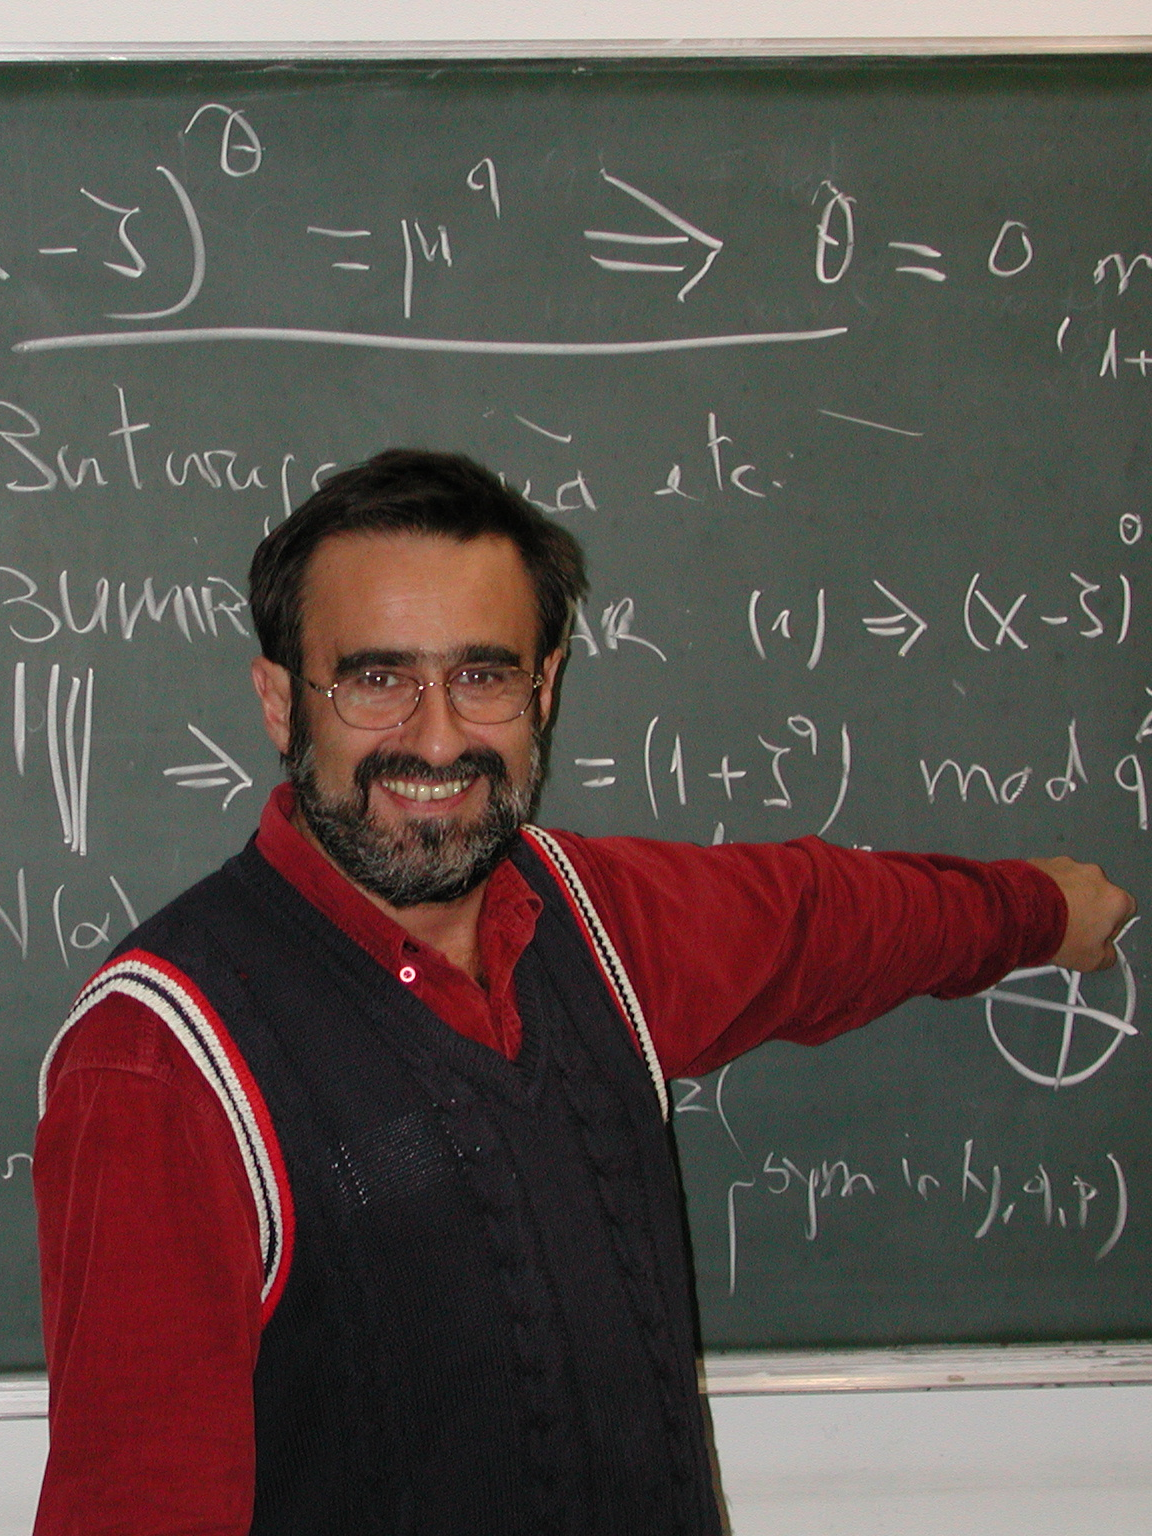
\includegraphics[width=5cm]{preda}
		\caption{Preda Mih\u{a}ilescu}
	\end{center}
\end{wrapfigure}
Die Catalan\footnote{nach Eugène Charles Catalan (1814-1894), ein belgischer Mathematiker}-Vermutung besagt, dass die Gleichung $x^a-y^b=1$ für $x,y \in \N$ und $a,b \in \Z_{\geq 2}$ nur die Lösung $3^2-2^3=1$ hat. Dies wurde 2002 von Preda Mih\u{a}ilescu\footnote{geb. 1955, ein in der Schweiz und in Deutschland wirkender rumänischer Mathematiker} bewiesen.

\begin{obs*}
	Der Abstand $x^2-y^3$ ist meistens \emph{viel größer} als 1 für hinreichend große $x,y \in \N$.
\end{obs*}

\begin{conj*}[Hall, 1969]
	Es gibt eine Konstante $C>0$ mit folgender Eigenschaft:\\
	Sind $x,y \in \N$ mit $x^3 \neq y^2$, dann ist
	\[ |x^2-y^2| > C x^\frac{1}{2}. \]
\end{conj*}

\begin{prop*}
	Es gibt eine Konstante $\tilde{c}$, sodass
	\[ |x^3-y^2| \leq \tilde{c} x^\frac{1}{2} \]
	unendlich viele Lösungen $(x,y) \in \N^2$ hat.
\end{prop*}

Betrachte
\[ \left( -5+ (u-3)^2 \right)^3 - (u^2+1) (u^2-9u+19)^2 = 27 (2u-11). \]
Wähle $u \in \Z$ mit $u^2+1 = 125v^2$, wobei $v\in \Z$ und $u \equiv 3 \bmod 5$. Sei
\begin{align*}
	x &= -1 + \frac{(u-3)^2}{5}\\
	y &= v(u^2-9u+19)
\end{align*}
Dann ist
\[ x^3-y^2 = \frac{27(2u-11)}{125}. \]
Es gilt
\begin{align*}
	\frac{|x^3-y^2|}{\sqrt{x}} &= \frac{27 |2u-11| \sqrt{5}}{125 \sqrt{(u-3)^2-5}}\\
	&\overset{u \to \infty}{\longrightarrow} \frac{2 \cdot 27}{25 \cdot \sqrt{5}}
\end{align*}
Das heißt es gibt eine Folge von natürlichen Zahlen $(x_n,y_n)$ mit
\[ \frac{\left| x_n^3-y_n^2 \right|}{\sqrt{x_n}} \overset{n \to \infty}{\longrightarrow} \frac{54}{25 \sqrt{5}}. \]
	\chapter{Die $abc$-Vermutung}

1986: Masser\footnote{David Masser (geb. 1948), ein britischer Mathematiker} und Oesterlé\footnote{Joseph Oesterlé (geb. 1954), ein französischer Mathematiker} studieren die Gleichung
\[ a+b=c \]
in $a,b,c \in \N$.

\begin{obs*}
	\begin{itemize}
		\item Werden $a$ und $b$ durch hohe Potenzen von kleinen Primzahlen geteilt, dann gilt das für $c$ nicht.
		\item Sei $p_1,\dotsc,p_r$ die Menge von Primzahlen, die eine der Zahlen $a,b,c$ teilen. Dann ist $p_1 \dotsm p_r$ relativ groß im Vergleich zu $\max\{|a|,|b|,|c|\}$.
	\end{itemize}
\end{obs*}

\begin{exmp*}
	\begin{enumerate}[label={\roman*})]
		\item $2^4+3^3 = 16+27=43 \implies p_1p_2p_3 = 6 \cdot 43$
		\item Selbst experimentieren!
	\end{enumerate}
\end{exmp*}

\begin{defn*}[Radikal einer Zahl] \index{Radikal!einer Zahl}
	Sei $n \in \N$ mit Primfaktorzerlegung
	\[ n = p_1^{k_1} p_2^{k_2} \dotsm p_r^{k_r} \]
	mit $p_1 < p_2 < \dots < p_r$. Dann definieren wir das \emph{Radikal} von $n$ als 
	\[ \rad(n):= p_1 \dotsm p_r. \]
\end{defn*}

\begin{conj*}[$abc$-Vermutung]
	Seien $a,b,c \in \N$ mit $a+b=c$ und $\ggt(a,b,c)=1$. Dann gibt es für jedes $\epsilon > 0$ eine Konstante $C_0(\epsilon) > 0$ mit folgender Eigenschaft:\\
	Ist $c > C_0(\epsilon)$, dann ist 
	$$c < \rad(abc)^{1+\epsilon}.$$
\end{conj*}
\begin{rem*}\lecture{01.06.2021}
	Warum benötigen wir $+\epsilon$ in der Vermutung?\\
	Hierfür betrachten wir $a=1,b=3^{2^n}-1,c=3^{2^n}$. Dann ist $a+b=c$ mit $\ggt(a,b,c)=1$. Es gilt
	\[ 2^{n+1} \mid 3^{2^n}-1. \]
	Also
	\begin{align*}
		\rad(abc) &= \rad \left( \left( 3^{2^n}-1 \right) 3^n \right)\\
		&= \rad \left( 3^{2^n} -1 \right) \rad(3^n)\\
		&\leq \frac{3^{2^n}-1}{2^n} \cdot 3\\
		&\leq \frac{3c}{2^n}
	\end{align*}
	Es folgt also
	\[ c > \frac{2^n}{3} \rad(abc). \]
\end{rem*}

\subsubsection*{Was ist bekannt zur $abc$-Vermutung?}

\begin{thm*}[Stewart \& Kunrui Yu, 1991]
	Für jedes \( \epsilon>0 \) gibt es eine Konstante $C_0(\epsilon)$, sodass gilt: Sind $a,b,c \in \N$ mit $a+b=c$ und $\ggt(a,b,c)=1$, so ist
	\[ c < \max \left\{ C_0(\epsilon), e^{\rad(abc)^{\frac{1}{3}+\epsilon}} \right\}. \]
\end{thm*}

\begin{thm*}[Pastén, 2017]
	Für jedes $\epsilon>0$ gibt es eine Konstante $C_0(\epsilon)$ mit folgender Eigenschaft: Sind $a,b,c \in \N$ mit $a+b=c$ und $\ggt(a,b,c)=1$, so gilt
	\[ d(abc) < C_0(\epsilon) \cdot \rad(abc)^{\frac{8}{3}+\epsilon}, \]
	wobei $d$ die Teilerfunktion ist.
\end{thm*}

\begin{conj*}[Schwache $abc$-Vermutung]
	Es gibt eine Konstante $\gamma>0$, sodass für alle $a,b,c \in \N$ mit $a+b=c$ und $\ggt(a,b,c)=1$ gilt
	\[ c \leq \rad(abc)^\gamma. \]
\end{conj*}

2012 behauptete Mochizuki\footnote{Shin’ichi Mochizuki (geb. 1969), ein japanischer Mathematiker}, die $abc$-Vermutung könne mit einer von ihm entwickelten "interuniversellen Teichmüller-Theorie". Dies erregte viel Aufmerksamkeit, allerdings widerlegten 2018 Scholze\footnote{Peter Scholze (geb. 1987), ein deutscher Mathematiker} und Stix\footnote{Jakob Stix (geb. 1974), ein deutscher Mathematiker} die Beweisideen von Mochizuki.

\section{Folgerungen aus der $abc$-Vermutung}

%\subsection{Quadratfreie Werte von Polynomen}

\begin{defn*}[Quadratfreie Zahl]\index{Quadratfreie Zahl}
	Wir nennen eine natürliche Zahl $m \in \N$ \emph{quadratfrei}, falls für jede Primzahl $p$ mit $p \mid m$ zusätzlich $p^2 \nmid m$ gilt.
\end{defn*}

\begin{frage*}
	Für welche natürlichen Zahlen $n \in \N$ ist $ n^4+1 $ quadratfrei?
\end{frage*}

\begin{conj*}
	\[ \left| \left\{ 1 \leq n \leq X \mid n^4+1 \ \text{ist quadratfrei} \right\} \right| \cong X \prod_p \left( 1-\frac{C_p}{p} \right) \]
	mit 
	\[ C_p = \left| \left\{ n \bmod p^2 \mid p^2 \mid n^4+1 \right\} \right| \]
\end{conj*}

\begin{thm*}[Granville, 1998]
	Angenommen die $abc$-Vermutung gilt. Sei $f \in \Z[x]$. Dann nimmt $f$ die erwartete Zahl von quadratfreien Werten an.
\end{thm*}

\begin{thm*}[Poonen\protect\footnotemark{}, 2003]
	\footnotetext{Bjorn Poonen (geb. 1968), ein US-amerikanischer Mathematiker}
	Granvilles Satz gilt auch für Polynome in mehreren Variablen.
\end{thm*}

\begin{frage*}
	Bestimmt alle $m,n \in \N$ mit $n!+1=m^2$.
\end{frage*}

Lösungen, die wir kennen, sind beispielsweise \( 4!+1=5^2, 5!+^=11^2, 7!+1=71^2,\dots \)\\
Angenommen, $m,n \in \N$ mit $n!+1=m^2$. Dann gilt
\begin{align*}
	n! &= m^2-1 \\ &=(m-1)(m+1)
\end{align*}
Ist $n \geq 2$, dann sind $m-1$ und $m+1$ beide gerade und aus Primfaktoren $\geq n$ aufgebaut. Wir wissen
\begin{align*}
	\frac{m-1}{2}+1 = \frac{m+1}{2}
\end{align*}
Berechne
\[ \rad \left( \frac{m-1}{2} \cdot \frac{m+1}{2} \right) \leq \prod_{p \leq n} p.\]
Wenn die schwache $abc$-Vermutung mit einem $\gamma>0$ gilt, so erhalten wir
\begin{align*}
	\frac{m+1}{2} &< \left( \rad \left( \frac{m-1}{2} \frac{m+1}{2} \right) \right)^\gamma\\
	&\leq \left( \prod_{p \leq n} p \right)^\gamma
\end{align*}
Man kann zeigen
\[ \prod_{p \leq n}p < 4^n. \]
Daraus folgt
\[ \frac{\sqrt{n!}}{2} < \frac{m+1}{2} < 4^{\gamma n}. \]
Gilt die schwache $abc$-Vermutung, dann gibt es höchstens endlich viele Lösungen der Gleichung
\[ n!+1 = m^2. \]

\begin{conj*}[Schwache Hall-Vermutung]
	Sei $0 < \delta < \frac{1}{2}$. Dann gibt es höchstens endlich viele Paare $x,y \in \N$ mit
	\[ 0 < |x^3-y^2| < x^\delta. \]
\end{conj*}

\begin{thm*}
	Die $abc$-Vermutung impliziert die schwache Hall-Vermutung.
\end{thm*}

\begin{frage*}
	Gibt es unendlich viele Primzahlen $p$, sodass $2{p-1} \equiv 1 \bmod p^2$?
\end{frage*}

\begin{rem*}
	Ist $p$ ungerade, so gilt nach Eulers Satz
	\[ 2^{p-1} \equiv 1 \bmod p. \]
\end{rem*}

\begin{thm*}[Silverman\protect\footnotemark{}, 1988]
	\footnotetext{Joseph Hillel Silverman (geb. 1955), ein US-amerikanischer Mathematiker}
	Angenommen die $abc$-Vermutung gilt. Dann gibt es unendlich viele Primzahlen $p$ mit $2^{p-1} \not\equiv 1 \bmod p^2$.
\end{thm*}
	\chapter{Irrationale Zahlen}\lecture{08.06.2021}

Rationale Zahlen $\Q$: $\frac{a}{b}$ mit $a \in \Z$, $b \in \N$.\\
Irrationale Zahlen: $\R \setminus \Q$.

\begin{frage*}
	Wie erkennt man, ob eine reelle Zahl $\alpha \in \R$ rational ist?
\end{frage*}

\begin{exmp*}
	$\sqrt{15}$ ist irrational:
	\[ \sqrt{15} = \frac{p}{q},\ p,q \in \Z \implies 15q^2 - p^2 = 0 \]
	Diese Gleichung hat allerdings keine ganzzahlige Lösung mit $\ggt(p,q)=1$.
\end{exmp*}

\begin{lem}\autolabel
	Sei $F(x) = x^m + c_1x^{m-1} + \dots + c_{m-1}x + c_m \in \Z[x]$ mit $c_m \neq 0$. Angenommen $\alpha \in \R$ mit $F(\alpha) \neq 0$. Dann gilt entweder
	\begin{itemize}
		\item $\alpha \in \Z$ und $\alpha \mid c_m$
		\item[] oder
		\item $\alpha$ ist irrational.
	\end{itemize}
\end{lem}

\begin{cor*}
	Sei $m \in \N$ und $N \in \N$, sodass $N$ keine $m$-te Potenz einer natürlichen Zahl ist. Dann ist $\sqrt[m]{N}$ irrational.
\end{cor*}

\begin{frage*}
	Finden wir weitere Beispiele von irrationalen Zahlen?
\end{frage*}

\begin{thm}\autolabel
	$e = \sum_{k=0}^{\infty} \frac{1}{k!}$ ist irrational.
\end{thm}

Zahlen, von denen wir nicht wissen, ob sie irrational sind:
\begin{itemize}
	\item Eulersche Konstante $\gamma = \lim_{n \to \infty} \left( 1 + \frac{1}{2} + \dots + \frac{1}{n} - \log n \right)$
	\item $e \cdot \pi,\ e + \pi$
	\item \( \sum_{k=1}^\infty \frac{1}{k!+1} \) (Frage von Erdős\footnote{Paul Erdős (1913-1996), ein ungarischer Mathematiker})
\end{itemize}

\begin{thm}\autolabel
	Sei $a \in \Q \setminus \{0\}$. Dann ist $e^a$ irrational.
\end{thm}

\begin{thm}\autolabel
	$\pi^2$ ist irrational (und damit auch $\pi$).
\end{thm}

\begin{defn*}[Legendre Polynom] \index{Legendre Polynom}
	Sei $m \in \Z_{\geq 0}$. Wir nennen
	\[ P_m(t) := \frac{1}{m!} \left( \frac{d}{dt} \right)^m \big( t^m (1-t)^m \big) \]
	das $m$-te \emph{Legendre Polynom}.
\end{defn*}

\begin{exmp*}
	$P_0(t)=1$\\
	$P_1(t) = \frac{d}{dt} \big( t(1-t) \big) = 1-2t$\\
	$P_2(t) = 1-6t+6t^2$
\end{exmp*}

\begin{lem}\autolabel
	Sei $m \in \Z_{\geq 0}$. Dann ist $P_m(t) \in \Z[t].$
\end{lem}

\begin{lem}\autolabel
	Sei $n \in \Z_{\geq 0}$. Dann ist
	\[ \pi \int_{0}^{1} t^n \sin(\pi t) \ dt \]
	ein Polynom in $\frac{1}{\pi^2}$ mit ganzzahligen Koeffizienten von Grad $\leq \left\lfloor \frac{n}{2} \right\rfloor$, das heißt es gibt ein $g \in \Z[x]$ mit \( \grad g \leq \left\lfloor \frac{n}{2} \right\rfloor \) und
	\[ \pi \int_{0}^{1} t^n \sin(\pi t) \ dt = g \left(\frac{1}{\pi^2}\right). \]
\end{lem}

\begin{lem*}
	Sei $n \in \Z_{\geq 0}$, $a \in \R\setminus\{0\}$. Dann gibt es Polynome $A_n(x), B_n(x) \in \Z[x]$ von Grad $\leq n$ mit
	\[ a \int_{0}^{1} t^n e^{at} \ dt = A_n \left( \frac{1}{a} \right) + B_n \left( \frac{1}{a} \right) e^a. \]
\end{lem*}

\section{Transzendente Zahlen}

\begin{defn*}[transzendente Zahlen]\index{transzendente Zahlen}
	Wir nennen $\alpha \in \R$ \emph{transzendent}, falls $\alpha$ keine Nullstelle eines Polynoms $P(x) \in \Z[x]\setminus\{0\}$ ist. Ist $\alpha$ nicht transzendent nennen wir es \emph{algebraisch}.
\end{defn*}

\begin{rem*}
	$\Q \subset \{\text{algebraische Zahlen}\} \subset \R$
\end{rem*}

\begin{thm}\autolabel
	Die reelle Zahl 
	\( \alpha = \sum_{k=0}^\infty \frac{1}{2^{k!}} \)
	ist transzendent.
\end{thm}

Beispiele von transzendenten Zahlen:
\begin{itemize}
	\item \( \sum_{k=0}^\infty \frac{1}{2^{2^k}} \) (Mahler\footnote{Kurt Mahler (1903-1988), ein deutschstämmiger britischer Mathematiker} 1930)
	\item \( \sum_{k=1}^\infty 2^{-k^2} \) (Nishioka\footnote{Kumiko Nishioka (geb. 1954), ein japanischer Mathematiker} \& Duveney 1996)
	\item $\pi$ ist transzendent (Hermite\footnote{Charles Hermite (1822-1901), ein französischer Mathematiker} 1873)
	\item $e$ ist transzendent (Lindemann\footnote{Carl Louis Ferdinand Lindemann (1852-1939), ein deutscher Mathematiker} 1882)
\end{itemize}
	\chapter{Charaktere und Gauß-Summen}
\lecture{11.06.2021}
\section{Charaktere}

\begin{idee*}
	Wir wollen für eine endliche abelsche Gruppe $G$ Gruppenhomomorphismen
	\[ \chi: G \to \C^* \]
	studieren. Dabei liegt unser Fokus zunächst auf $G \cong (\Z/m\Z)^*$ für ein $m \in \N$.
\end{idee*}

\begin{defn*}[Charakter] \index{Charakter}
	Sei $m \in \N$. Ein \emph{multiplikativer Charakter modulo \( \emph{m} \)} ist ein Gruppenhomomorphismus
	\[ \chi: (\Z/m\Z)^* \to \C^*, \]
	sodass gilt $\chi(ab) = \chi(a)\chi(b)\ \foralll a,b \in (\Z/m\Z)^*$.
\end{defn*}

\begin{exmp*}
	Ist $p$ prim, dann ist das Legendre-Symbol
	\[ \left(\frac{\cdot}{p}\right): (\Z/p\Z)^* \to \{\pm 1\} \]
	ein multiplikativer Charakter modulo $p$.
\end{exmp*}

\begin{frage*}
	Wie können wir einen multiplikativen Charakter modulo $m$ zu einer Funktion \[ \chi: \Z \to \C \] erweitern?
\end{frage*}

\begin{defn*}[Dirichlet-Charakter] \index{Charakter!Dirichlet-Charakter}
	Sei $n \in \N$. Ein \emph{Dirichlet-Charakter modulo $\emph{m}$} ist eine Funktion
	\[ \chi: \Z \to \C \]
	mit den Eigenschaften
	\begin{enumerate}[label={\roman*})]
		\item $\chi(a) = 0 \iff \ggt(a,m)>1$.
		\item Ist $a \equiv b \bmod m$, dann gilt $\chi(a)=\chi(b)$.
		\item Für $a,b \in \Z$ gilt $\chi(a)\chi(b)=\chi(ab)$.
	\end{enumerate}
\end{defn*}

\begin{rem*}
	Ist $\chi : Z \to \C$ ein Dirichlet-Charakter modulo $m$, so induziert $\chi$ einen multiplikativen Charakter $\tilde{\chi}$ modulo $m$ durch
	\[ \tilde{\chi}: (\Z/m\Z)^* \to \C^*,\quad \bar{a} \mapsto \chi(a). \]
\end{rem*}

\begin{exmp*}
	\begin{enumerate}[label={\roman*})]
		\item Für $p$ prim ist das Legendre-Symbol $\left(\frac{\cdot}{p}\right)$ ein Dirichlet-Charakter modulo $p$.
		\item Sei $m \in \N$ und definiere $\chi_0: \Z \to \C$ durch
			\[ \chi_0(a) = \begin{cases}
				0 &\ggt(a,m)>1\\
				1 &\ggt(a,m)=1
			\end{cases} \]
			Dann ist $\chi_0$ ein Dirichlet-Charakter modulo $m$. Wir nennen $\chi_0$ den \emph{Hauptcharakter} modulo $m$.
	\end{enumerate}
\end{exmp*}

Wir wollen nun erste Eigenschaften von Dirichlet-Charakteren betrachten.

\begin{lem}\autolabel
	Sei $m \in \N$ und $\chi$ ein Dirichlet-Charakter modulo $m$. Dann gilt
	\begin{enumerate}[label={\roman*})]
		\item $\chi(1)=1$.
		\item Ist $a \in \Z$ mit $\ggt(a,m)=1$, so ist $\chi(a)$ eine $\varphi(m)$-te Einheitswurzel, d.h. $\chi(a)^{\varphi(m)}=1$.
		\item Die Funktion $\bar{\chi}: \Z \to \C$ definiert durch
			\[ \bar{\chi}(a=) = \overbar{\chi(a)} \]
			ist wieder ein Dirichlet-Charakter.
	\end{enumerate}
\end{lem}

\begin{rem*}
	Das Produkt von zwei Dirichlet-Charakteren modulo $m$ ist wieder ein Dirichlet-Charakter modulo $m$.\\
	Genauer gilt
\end{rem*}

\begin{lem}\autolabel
	Sei $m \in \N$. Dann ist die Menge aller Dirichlet-Charaktere modulo $m$, schreibe $\Ccal_m$, eine endliche abelsche Gruppe unter der Multiplikation,
	\[ \chi_1 \cdot \chi_2(a) = \chi_1(a) \chi_2(a) \ \foralll a \in \Z. \]
\end{lem}

\begin{frage*}
	Wie viele verschiedene Dirichlet-Charaktere gibt es?
\end{frage*}

\begin{lem}\autolabel
	Seien $m,d \in \N$ mit $\ggt(m,d)=1$ und $d \not\equiv1 \bmod m$. Dann gibt es einen Dirichlet-Charakter $\chi$ modulo $m$ mit $\chi(d) \neq 1$.
\end{lem}

\begin{exmp*}
	$m = 5$. 2 ist eine Primitivwurzel modulo 5. Die Funktion
	\[ \chi(a) = \begin{cases}
		0 &\ggt(a,5)>1\\
		e^{2\pi i \frac{c}{4}} &\ggt(a,5)=1,\ a \equiv 2^c \bmod 5
	\end{cases} \]
	ist ein Dirichlet-Charakter modulo 5. Explizit gilt $\chi(1)=1, \chi(2)=i,\chi(3)=-i,\chi(4)=-1$ und damit
	\[ \chi(1)+\chi(2)+\chi(3)+\chi(4)=0. \]
\end{exmp*}

\begin{frage*}
	Gilt dies auch allgemein?
\end{frage*}

\begin{thm}\autolabel
	Sei $m \in \N$ und $\Ccal_m$ die Gruppe der Dirichlet-Charaktere modulo $m$, $\chi \in \Ccal_m$ und $a \in \Z$ mit $\ggt(a,m)=1$. Dann gilt
	\begin{enumerate}[label={\roman*})]
		\item \[ \sum_{\chi \in \Ccal_m} \chi(a) = \begin{cases}
				|\Ccal_m| &a \equiv 1 \bmod m\\
				0 &a \not\equiv 1 \bmod m
			\end{cases} \]
		\item \[ \sum_{\substack{1 \leq a \leq m\\\ggt(a,m)=1}} \chi(a) = \begin{cases}
				\varphi(m) &\chi = \chi_0\\
				0 &\chi \neq \chi_0
			\end{cases} \]
		\item \[ |\Ccal_m| = \varphi(m). \]
	\end{enumerate}
\end{thm}
\section{Gauß-Summen}\lecture{15.06.2021}

Sei $m \in \N$. Bisher haben wir Charaktere
\[ \tilde{\chi}: (\Z/m\Z)^* \to \C^* \]
studiert, die multiplikativen Charaktere modulo $m$. Wir betrachten nun die additive Gruppe $\Z/m\Z$ und  Gruppenhomomorphismen
\[ (\Z/m\Z,+) \to (\C^*,\cdot). \]

\begin{frage*}
	Welche Form haben "additive Charaktere" modulo $m$?
\end{frage*}

Sei 
\[ f: (\Z/m\Z,+) \to (\C^*,\cdot) \]
ein Gruppenhomomorphismus. Dann gilt
\[ f(0) = 1 \]
\[ f(1)^m = f(m) = f(0) = 1, \]
d.h. $f(1)$ ist eine $m$-te Einheitswurzel. Es gibt also $a \in \Z$ mit
\[ f(1) = e^{2\pi i \frac{a}{m}}. \]
Dann gilt allgemein für $c \in \Z/m\Z$
\[ f(c) = f(1)^c = e^{2\pi i \frac{ac}{m}} \]

\begin{notat*}
	Für $x \in \R$ schreiben wir im Folgenden
	\[ e(x) = e^{2\pi i x}. \]
\end{notat*}

\begin{frage*}
	Wie sehen die Interaktionen zwischen additiven und multiplikativen Charakteren modulo $m$ aus?
\end{frage*}

Wir betrachten nun den Fall, in dem $m=p$ prim ist.

\begin{defn*}[Gauß-Summe]\index{Gauß-Summe}
	Sei $p$ eine Primzahl und $\chi$ ein Dirichlet-Charakter modulo $p$ mit $\chi \neq \chi_0$. Für $a \in \Z$ definieren wir die \emph{Gauß-Summen}
	\[ g_a(\chi) = \sum_{t=0}^{p-1} \chi(t) e\left( \frac{at}{p} \right), \]
	\[ g_a(\chi_0) = \sum_{t=0}^{p-1} e\left( \frac{at}{p} \right). \]
\end{defn*}

\begin{notat*}
	Für $a=1$ schreibe auch $g_1(\chi) = g(\chi)$.
\end{notat*}

\begin{rem*}
	\begin{enumerate}[label={\roman*})]
		\item Ist $a \equiv b \bmod p$, so gilt
			\[ g_a(\chi) = g_b(\chi) \]
			für alle Dirichlet-Charaktere modulo $p$.
		\item Für den Hauptcharakter $\chi_0$ berechnen wir
			\begin{align*}
				g_a(\chi_0) &= \sum_{t=0}^{p-1} e\left( \frac{at}{p} \right)\\
				&= \begin{cases}
					p\quad &p \mid a\\
					0 &p \nmid a
				\end{cases}
			\end{align*}
	\end{enumerate}
\end{rem*}

\begin{frage*}
	Wie funktioniert die Berechnung von Gauß-Summen für allgemeine Charaktere $\chi$?
\end{frage*}

Zur Beantwortung dieser Frage betrachten wir zunächst die Reduktion auf den Fall $a=1$, d.h. $g_1(\chi) = g(\chi)$.

\begin{lem}\autolabel
	Sei $p$ prim, $a \in \Z$ und $\chi$ ein Dirichlet-Charakter modulo $p$ mit $\chi \neq \chi_0$. Falls $p \nmid a$ sei $a^* \in \Z$ mit $aa^* \equiv 1 \bmod p$. Dann gilt
	\[ g_a(\chi) = \begin{cases}
		0 &p \mid a\\
		\chi(a^*)g(\chi) &p \nmid a
	\end{cases} \]
\end{lem}

\begin{frage*}
	Welche Größenordnung könnte man für $g(\chi)$ für große Primzahlen $p$ erwarten?
\end{frage*}

\begin{idee*}
	Falls die Summanden $\chi(t) e\left( \frac{t}{p} \right)$ zufällig auf dem Einheitskreis verteilt wären, so könnten wir für ein großes $p$
	\[ |g(\chi)| \sim \sqrt{p} \]
	erwarten (square root cancellation).
\end{idee*}

\begin{thm}\autolabel
	Sei $p$ prim und $\chi \neq \chi_0$ ein Dirichlet-Charakter modulo $p$. Dann gilt
	\[ |g(\chi)| = \sqrt{p}. \]
\end{thm}

Im Spezialfall, dass $\chi = \left(\frac{\cdot}{p}\right)$ das Legendre-Symbol ist, können wir noch etwas mehr sagen:

\begin{thm}\autolabel
	Sei $p>2$ prim und $\left(\frac{\cdot}{p}\right)$ das Legendre-Symbol. Dann gilt
	\[ g(\chi)^2 = (-1)^{\frac{p-1}{2}}p. \]
\end{thm}

Eine erste Anwendung von Gauß-Summen ist der Beweis des quadratischen Reziprozitätsgesetzes. eine weitere ist die

\subsection{Arithmetik in Kreisteilungskörpern}

Sei $p$ eine Primzahl und $\zeta = e\left( \frac{1}{p} \right) = e^{\frac{2\pi i}{p}}$. Dann ist
\[ \Q(\zeta) = \big\{ a_0 + a_1\zeta + \dots + a_{p-2}\zeta^{p-2} \mid a_0,a_1,\dotsc,a_{p-2} \in \Q \big\} \subset \C \]
ein Körper und
\[ \Z[\zeta] = \big\{ a_0 + a_1\zeta + \dots + a_{p-2}\zeta^{p-2} \mid a_0,a_1,\dotsc,a_{p-2} \in \Z \big\} \]
ein Teilring.

\begin{rem*}
	Es gilt
	\[ 1 + \zeta + \dots + \zeta^{p-1} = \sum_{t=0}^{p-1} e\left( \frac{t}{p} \right) = 0. \]
	Also können wir $\zeta^{p-1}$ schreiben als
	\[ \zeta^{p-1} = -1 - \zeta - \zeta^2 - \dots - \zeta^{p-2} \in \Z[\zeta]. \]
\end{rem*}

\begin{notat*}
	Sind $\alpha,\beta \in \Z[\zeta]$ und $q \in \Z$ eine weitere Primzahl, so schreiben wir 
	\[ \alpha \equiv \beta \bmod q \]
	falls $\alpha-\beta = q\gamma$ mit $\gamma \in \Z[\zeta]$ ist.
\end{notat*}

\begin{exmp*}
	$p=5,\ q = 7,\ 7 + \zeta + 8\zeta^2 \equiv \zeta + \zeta^2 \bmod 7$
\end{exmp*}

\begin{lem}\autolabel
	Sei $q \neq p$ eine weitere Primzahl und $m,n \in \Z$ mit $m \equiv n \bmod q$ im Ring $\Z[\zeta]$. Dann gilt bereits $m-n = q \cdot c$ mit einem $c \in \Z$.
\end{lem}
	
	
	
	
	
	\pagestyle{plain}
%	\appendix
%	\renewcommand{\appendixtocname}{Anhang}
%	\addappheadtotoc
	\printindex
\end{document}